\documentclass[10pt,a4paper,twoside,openright]{memoir}
\usepackage[utf8]{inputenc}
\usepackage[ngerman,english]{babel}

% ----- pgfplots -----
\usepackage{femtikz} % pgfplots, tikz, graphicx
\usetikzlibrary{babel}
\usepgfplotslibrary{groupplots}
\usepgfplotslibrary{colorbrewer}
\pgfplotsset{compat=1.9} % colorbar style ylabel
% \selectcolormodel{rgb}
% \usetikzlibrary{external}
% \tikzexternalize[prefix=tikz/]
% environment for tikzpicture containing legend only
% see: http://tex.stackexchange.com/questions/54794/using-a-pgfplots-style-legend-in-a-plain-old-tikzpicture/54834#54834)
% argument #1: any options
\newenvironment{customlegend}[1][]{
  \begingroup
  % inits/clears the lists (which might be populated from previous axes):
  \csname pgfplots@init@cleared@structures\endcsname
  \pgfplotsset{#1}%
}{
  % draws the legend:
  \csname pgfplots@createlegend\endcsname
  \endgroup
}
% makes \addlegendimage available (typically only available within an axis environment):
\def\addlegendimage{\csname pgfplots@addlegendimage\endcsname}
\def\addlegendentry{\csname pgfplots@addlegendentry\endcsname}



% Style to select only points from #1 to #2 (inclusive)
% see: https://tex.stackexchange.com/questions/199376/how-to-plot-the-first-n-rows-of-a-table-using-pgfplots
\pgfplotsset{select coords between index/.style 2 args={
  x filter/.code={
    \ifnum\coordindex<#1\def\pgfmathresult{}\fi
    \ifnum\coordindex>#2\def\pgfmathresult{}\fi
  }
}}

% ----- formatting -----
\usepackage{titling}
\usepackage{enumitem} % resume
\usepackage{subcaption}
\usepackage[binary-units=true]{siunitx}
\usepackage{perpage}
\MakePerPage{footnote}
\usepackage[
  colorlinks,linkcolor=blue,urlcolor=blue,citecolor=blue % suggestion of wolfgang
  % colorlinks,linkcolor=black,urlcolor=black,citecolor=black % print version
]{hyperref}
\OnehalfSpacing % memoir
\nouppercaseheads % memoir
\newcommand{\h}{\textit{h}}
\newcommand{\p}{\textit{p}}
\newcommand{\hp}{\textit{hp}}

\newcommand{\dealii}{\texttt{deal.II}}
\newcommand{\pforest}{\texttt{p4est}}
\newcommand{\petsc}{\texttt{PETSc}}
\newcommand{\trilinos}{\texttt{Trilinos}}
\newcommand{\epetra}{\texttt{Epetra}}
\newcommand{\aztecoo}{\texttt{AztecOO}}
\newcommand{\ml}{\texttt{ML}}
\newcommand{\xsdk}{\texttt{xSDK}}

\newcommand{\opencascade}{\texttt{OpenCASCADE}}
\newcommand{\opensalome}{\texttt{OpenSALOME}}
\newcommand{\fftw}{\texttt{FFTW}}
\newcommand{\mofem}{\texttt{MoFEM}}
\newcommand{\phg}{\texttt{PHG}}
\newcommand{\phaml}{\texttt{PHAML}}


% ----- math -----
\usepackage{amsmath,amsfonts,amssymb}
\usepackage{mathtools} % \coloneqq
\usepackage{isomath} % \vectorsym, \matrixsym, \tensorsym
\DeclareMathOperator{\Froude}{Fr}
\DeclareMathOperator{\Mach}{Ma}
\DeclareMathOperator{\Prandtl}{Pr}
\DeclareMathOperator{\Reynolds}{Re}
\DeclareMathOperator{\Strouhal}{St}

\newcommand{\differential}[1]{\ensuremath{\mathop{}\!\mathrm{d}#1}}
\newcommand{\tuple}[1]{\ensuremath{\vectorsym{#1}}}
\renewcommand{\vec}[1]{\ensuremath{\vectorsym{#1}}}
\newcommand{\mat}[1]{\ensuremath{\matrixsym{#1}}}
\newcommand{\ten}[1]{\ensuremath{\tensorsym{#1}}}

\newcommand{\source}[1]{\ensuremath{\dot{#1}'''}}

\newcommand{\cellsp}[1]{\ensuremath{\mathbb{T}^p_{\text{#1}}}}

% ----- glossary -----
\usepackage[automake,style=super]{glossaries-extra}
\makeglossaries
\newabbreviation{api}{API}{application programming interface}
\newabbreviation{cuda}{CUDA}{Compute Unified Device Architecture}
\newabbreviation{mpi}{MPI}{Message Passing Interface}
\newabbreviation{openacc}{OpenACC}{Open Accelerators}
\newabbreviation{openmp}{OpenMP}{Open Multi-Processing}
\newabbreviation{tbb}{TBB}{Threading Building Blocks}

\newabbreviation{cfd}{CFD}{computational fluid dynamics}

\newabbreviation{hpc}{HPC}{high-performance computing}

\newabbreviation{fdm}{FDM}{finite difference method}
\newabbreviation{fvm}{FVM}{finite volume method}
\newabbreviation[plural={FEM}, \glsshortpluralkey={FEM}]{fem}{FEM}{finite element method}
\newabbreviation{fft}{FFT}{fast Fourier transformation}
\newabbreviation{lbm}{LBM}{lattice Boltzmann method}

\newabbreviation[longplural={degrees of freedom}]{dof}{DoF}{degree of freedom}

\newabbreviation{cg}{CG}{continuous Galerkin}
\newabbreviation{dg}{DG}{discontinuous Galerkin}

\newabbreviation{amg}{AMG}{algebraic multigrid}
\newabbreviation{gmg}{GMG}{geometric multigrid}

% ----- bibliography -----
\usepackage[backend=biber, style=authoryear, labelnumber, defernumbers = true]{biblatex}
\DefineBibliographyStrings{english}{citedas = {hereafter}}
\addbibresource{misc/bibliography.bib}
\addbibresource{misc/references.bib}
% Two bibliographies with different styles and sortings for publications and weblinks, respectively.
%   based on: https://tex.stackexchange.com/questions/299064/
%             https://tex.stackexchange.com/questions/452170/

\DeclareSourcemap{
  % append keywords to identify different bibliography entries.
  \maps[datatype=bibtex, overwrite]{
    \map{
      \perdatasource{bibliography.bib}
      \step[fieldset=KEYWORDS, fieldvalue=primary] % do not append!
      % print the following fields only if there is no doi
      \step[fieldsource=doi,final]
      \step[fieldset=url,null]
      \step[fieldset=urldate,null]
      \step[fieldset=isbn,null]
      \step[fieldset=issn,null]
    }
    \map{
      \perdatasource{references.bib}
      \step[fieldset=KEYWORDS, fieldvalue=secondary] % do not append!
      % print the following fields only if there is no doi
      \step[fieldsource=doi,final]
      \step[fieldset=url,null]
      \step[fieldset=urldate,null]
      \step[fieldset=isbn,null]
      \step[fieldset=issn,null]
    }
  }
}

\DeclareFieldFormat{labelnumberwidth}{\mkbibbrackets{#1}}
\defbibenvironment{bibliographyNUM}
{\list
  {\printtext[labelnumberwidth]{%
      \printfield{prefixnumber}%
      \printfield{labelnumber}}}
  {\setlength{\labelwidth}{\labelnumberwidth}%
    \setlength{\leftmargin}{\labelwidth}%
    \setlength{\labelsep}{\biblabelsep}%
    \addtolength{\leftmargin}{\labelsep}%
    \setlength{\itemsep}{\bibitemsep}%
    \setlength{\parsep}{\bibparsep}}%
  \renewcommand*{\makelabel}[1]{\hss##1}}
{\endlist}
{\iffieldequalstr{labeldatesource}{url}{\clearfield{labelyear}}{}% clear labelyear if no date specified
\item}

\assignrefcontextkeyws[sorting=none]{secondary}



% modify cite and textcite macros for 'authoryear'
%   based on: https://github.com/plk/biblatex/blob/dev/tex/latex/biblatex/cbx/authoryear.cbx

\newbibmacro*{cite}{%
  \ifkeyword{secondary}
  % modification for additional bibliography
  {\mkbibbrackets{\printtext[bibhyperref]{%
    \printfield{labelprefix}\printfield{labelnumber}}}}
  % original macro
  {\iffieldundef{shorthand}
  {\ifthenelse{\ifnameundef{labelname}\OR\iffieldundef{labelyear}}
    {\usebibmacro{cite:label}%
      \setunit{\printdelim{nonameyeardelim}}}
    {\printnames{labelname}%
      \setunit{\printdelim{nameyeardelim}}}%
    \usebibmacro{cite:labeldate+extradate}}
  {\usebibmacro{cite:shorthand}}}}

\newbibmacro*{textcite}{%
  \ifkeyword{secondary}
  % modification for additional bibliography
  {\mkbibbrackets{\printtext[bibhyperref]{%
    \printfield{labelprefix}\printfield{labelnumber}}}}
  % original macro
  {\ifnameundef{labelname}
  {\iffieldundef{shorthand}
    {\usebibmacro{cite:label}%
      \setunit{%
        \global\booltrue{cbx:parens}%
        \printdelim{nonameyeardelim}\bibopenparen}%
      \ifnumequal{\value{citecount}}{1}
      {\usebibmacro{prenote}}
      {}%
      \usebibmacro{cite:labeldate+extradate}}
    {\usebibmacro{cite:shorthand}}}
  {\printnames{labelname}%
    \setunit{%
      \global\booltrue{cbx:parens}%
      \printdelim{nameyeardelim}\bibopenparen}%
    \ifnumequal{\value{citecount}}{1}
    {\usebibmacro{prenote}}
    {}%
    \usebibmacro{citeyear}}}}



% --- document information ---
\author{Marc Fehling}
\title{Algorithms for massively parallel generic \hp-adaptive finite element methods}
\date{April 2020}



\begin{document}
  \begin{titlingpage}
    \begin{center}
      \vspace*{\fill}
      
\includegraphics[width=.75\textwidth]{logos/BUW_Logo-schwarz.eps}\bigskip
      \vspace*{\fill}\par
      {\Huge \thetitle\bigskip\par}
      \vspace*{\fill}\par
      {\Large School of Architecture and Civil Engineering\bigskip\par}
      {\Large Dissertation for the acquisition of a doctorate\\(Dr.-Ing.)\bigskip\par}
      {\Large submitted by\bigskip\par}
      {\LARGE \theauthor\par}
      {\Large from Lübbecke\bigskip\par}
      {\Large Wuppertal, \thedate\bigskip\bigskip\par}
    \end{center}
  \end{titlingpage}
  
  
  
  \frontmatter
  
  \thispagestyle{plain}
  \begin{abstract}
  Abstract.
  
  \dealii{}\footnote{\url{https://www.dealii.org}} library.
\end{abstract}
  \clearpage
  
  \thispagestyle{plain}
  \begin{otherlanguage}{ngerman}
    \begin{abstract}
Für die numerische Lösung partieller Differentialgleichungen sind effiziente Algorithmen erforderlich, um Probleme auf einer wirtschaftlich tragbaren Zeitskala zu lösen.
Im Allgemeinen ist dies durch die Anpassung der Diskretisierungsauflösung an das untersuchte Problem sowie durch die Ausnutzung der Hardwarespezifikationen möglich.
Für die letztere Kategorie spielt die Parallelisierung eine große Rolle für moderne Mehrkern- und Mehrknotenarchitekturen, insbesondere im Kontext des Hochleistungsrechnens.

Mit Hilfe von Finite-Elemente-Methoden werden Lösungen durch Diskretisierung des assoziierten Funktionsraums mit stückweisen Polynomen approximiert. Bei \hp-adaptiven Methoden können die Polynomgrade dieser Basisfunktionen auf lokal verfeinerten Gittern variieren.

In dieser Dissertation werden Algorithmen und Datenstrukturen vorgestellt, die für generische \hp-adaptive Finite-Elemente-Software benötigt werden und sowohl für kontinuierliche als auch diskontinuierliche Galerkin-Verfahren auf Systemen mit verteiltem Speicher anwendbar sind. Sowohl der Funktionsraum als auch das Gitter können während des Lösungsprozesses dynamisch angepasst werden.

Im Besonderen erläutert werden die eindeutige Nummerierung von Freiheitsgraden mit kontinuierlichen Galerkin-Verfahren, die Kommunikation von Daten variabler Größe und die Lastenverteilung.
Außerdem werden Strategien zur Bestimmung des Adaptierungstyps auf der Grundlage von Fehlerprognosen sowie Glattheitsschätzungen vorgestellt, die über die Zerfallsrate von Koeffizienten aus Reihenentwicklungen nach Fourier und Legendre bestimmt werden. Dabei werden sowohl Verfeinerung als auch Vergröberung berücksichtigt.

Eine Referenzimplementierung erfolgt in der Open-Source-Bibliothek \dealii{}\footnote{\url{https://www.dealii.org}} und wird auf das Laplace-Problem auf einem Gebiet mit einer einschneidenden Ecke angewandt, die eine Singularität hervorruft. Anhand dieses Beispiels werden die Vorteile der \hp{}-adaptiven Methoden hinsichtlich der Fehlerkonvergenz und die Skalierbarkeit der präsentierten Algorithmen auf bis zu 49.152 \texttt{MPI}-Prozessen demonstriert.
\end{abstract}
  \end{otherlanguage}
  \clearpage
  
  \thispagestyle{plain}
  \section*{Acknowledgements}
\addcontentsline{toc}{chapter}{Acknowledgements}

The investigations carried out in this dissertation were performed with the \dealii{} library, and I cannot thank the whole \dealii{} community enough for all their support. In particular, I would like to express my gratitude towards Prof.\ Dr.\ Wolfgang Bangerth for hosting me during a seven month research stay at the Colorado State University and for reviewing this thesis, as well as Peter Munch for his interest in both my work and its expansion and for proofreading. I would like to also thank Dr.\ Denis Davydov and Dr.\ Martin Kronbichler for their collaboration, as well as Graham Harper and Sean McGovern for lots of \dealii{} related discussions.

I like to emphasize my gratitude to Prof.\ Dr.\ Armin Seyfried as the head of my home institute and my supervisor Prof.\ Dr.\ Lukas Arnold for making my PhD project possible. I am grateful for their support and encouragement, especially in spending about half a year abroad which allowed me to make huge progress in the project that was mandatory for its completion.

Furthermore, I wish to thank all the people I had the pleasure of meeting and working with during my time at the Forschungszentrum Jülich and the Bergische Universität Wuppertal. Thanks to Dr.\ Anne Kathrin Küsters and My Linh Würzburger for helpful discussions about numerics and programming and for proofreading, as well as Dr.\ Alexander Belt for his continuous motivation. In addition, I would also like to mention Dr.\ Erik Andresen, Anna Braun, Patrick Lauer, Jette Schumann, Corinna Trettin, and Ashish Vinayak, who became close friends.

Last, I am grateful to all friends and family for their continuous support on my journey. Be it through hiking adventures, joint sports activities such as running, cycling and swimming, riding roller coasters, attending concerts or simply by spending time together in any other possible way. It is impossible to mention all the people I have in mind here, and I hope that you, as a reader of these lines, feel addressed and associate pleasant memories in the same way as I do. I am grateful to have spent these moments with you and look forward to many more to come. Thank you.

  \clearpage
  
  \begin{KeepFromToc} % memoir
    \tableofcontents
  \end{KeepFromToc}
  \cleardoublepage
  
  \listoffigures
  
  \printglossary[type=\acronymtype, title={List of Abbreviations}]
  
  
  
  \mainmatter
  
  \chapter{Introduction}
\label{ch:introduction}

\todo{Introduction:}
\begin{itemize}
  \item Need for new computational methods (adaptive)
  \item Statistics on usage of FDS? (literatur aus bennis diss?)
  
  \item Latest catastrophes: tower, Düsseldorf
  \item ... help to .. catastrophes by giving hints on placements of safety measures.
\end{itemize}

Recent advancements in computer technology allows us to solve problems with billions of unknowns. However, raw computing power does not mean we can use it without further ado. The keys to efficiency are algorithms that exploit the hardware structure and focus resources on critical operations.

For currently common multi-processor systems, algorithms for parallelization need to be supplied . These methods depend on the hardware architecture, and especially large-scale supercomputers with distributed memory access benefit from this method.

Lots of \glspl{api} exist for these purposes, that allow users to take opportunity of already implemented ideas.

For machines with shared memory access, \glsdesc{openmp}\glsunset{openmp} \parencite{openmp50} and \glsdesc{tbb}\glsunset{tbb} \parencite{tbb2018} with its work stealing policy are the most prominent approaches. IF architecture is distributed on nodes and thus have distributed memory access, the \glsdesc{mpi}\glsunset{mpi} \parencite{mpi31} will be used. A combination of both is possbile.

Further, recently streaming multiprocessor architecture have become more and more interest, that work on graphic accelerator cards (GPUS). \glsdesc{openacc}\glsunset{openacc} \parencite{openacc27} or nVidia's \glsdesc{cuda}\glsunset{cuda} \parencite{cuda10} can be used for that.

On the other hand, . adaptive

A combinatation of both hardware and .. software driven algorithms can be supplied. However, their combination is not trivial. 

"MPI remains the dominant library for production programming on large scale distributed memory machines."

Some typeof hardware-related 
To name a few, Hardware-related algorithms are parallelization, vectorization and limiting memory access, since it. In terms 


guarantee the full usage of all available resources. The key to use those ausnutzen fully are efficient algorithms that either fit to the hardware or distribute resources on computing intensive operations.

However, the key to use these structures efficientis to , and not computing power alone; (Erst) the combination with algorithms that use these structure efficiently offers a massive potential to reduce 




Some of them

parallelization, vectorization, limit memory access. adaptive methods

parallelization depending on hardware architecture: MPI for distributed memory, OpenMP for shared memory, OpenACC or nVidia CUDA for streaming multiprocessors on e.g. GPUs

adaptive methods to focus .


Each algorithm . The combination of both is more or less trivial.
On supercomputers
This thesis presents the combination of both parallelization on distributed hardware architecture, and hp-adaptive methods.

For spatial discretizations we use . The \gls{fem}


This dissertation is not meant to be an in-depth guide for the creation of \gls{fem} software. We would rather like to emphasize on the basic ideas for parallel hp-adaptive \gls{fem} and point out programming challenges. We will provide an example implementation in the \dealii{} library, so that the reader is able to either embed our findings into his own \gls{fem} code or use the \dealii{} implementation right away.
  \chapter{Massively parallel \hp-adaptive \glsfmtlongpl{fem}}
\label{ch:parallel}

Text.



\section{Enumeration of \glsfmtlongpl{dof}}
\label{sec:enumeration}

Formulating and solving the system of linear equations requires an unique identification of all involved \glspl{dof} in the global mesh.

\Glspl{dof} are associated with mesh objects, i.e., vertices, edges, faces, and cells. If support points are located on interfaces between neighboring cells in the context of \gls{dg} methods, they are assigned separate \glspl{dof} on each cell. Thus, the enumeration of both \glspl{dof} and cells can happen analogously. However, \gls{cg} methods require that shared \glspl{dof} on interfaces between neighboring cells are unique. Thus, each \gls{dof} has to relate to a single cell, or in other words, will be owned by a single cell. This assignment is crucial for the preparation of relevant distributed data structures.

%Depending on which Galerkin method has been picked, we need to ... .
%Continous Galerkin methods require a unique identification of \glspl{dof} on interfaces between cells, because of the continuity requirement on the solution.

The latter scenario poses challenges in the enumeration of \glspl{dof} when considering either parallelization or \hp-adaptive methods, let alone a combination of both. A first attempt to cope with this problem would involve so called constraints: We enumerate all \glspl{dof} on each cell independently, but identify two similar \glspl{dof} as identical during the assembly of the equation systems. Although this approach would be easy to implement, we would needlessly add \gls{dof} duplicates to the equation system, sacrificing performance by wasting memory and computing time. We conclude that a unique enumeration of \glspl{dof} is mandatory for a robust \gls{fem} implementation for \gls{cg} methods.

Both \textcite{bangerth2012} and \textcite{bangerth2009} have dealt with \gls{dof} enumeration with parallelization and \hp-adaptive methods, respectively, and presented algorithms for each case, but the combination of both is not trivial. In this section, we will briefly summarize each implementation and present an enhanced algorithm in detail for the unique identification of \glspl{dof} for \gls{cg} methods with parallel \hp-adaptive methods.

In the following, all algorithms will be presented independently of the underlying data structures and should be easily applicable on any kind of existing \gls{fem} code. Results will be presented afterwards with our reference implementation in the \dealii{} library.

%A common approach to parallelization for cell based methods on distributed memory machines is to assign multiple cells to one process of that form a subdomain. Typically during the assembly of the equation system we need to the values of the surrounding cells. Thus, an extension of the subdomain by so called ghosts cells is required.

%When using continuous Galerkin methods on the other hand, \glspl{dof} are shares along interfaces between cells.

%However, a different way of enumerating \glspl{dof} has to be taken with parallel \gls{fem}. \textcite{bangerth2012} provided a

%For \hp-adaptive methods, cells with different finite elements assigned may neighbor each other. Thus, we may also encounter hanging nodes on neighboring cells as depicted in Fig.~\ref{fig:papaptivity} in addition to the ones arising from \h-adaptation.

%In the context of \gls{cg} methods, these hanging nodes from \p-adaptation need to comply to the continuity condition along the faces of a cell.

%For \hp-adaptive methods, cells with different finite elements assigned may neighbor each other. Thus, we may also encounter hanging nodes on neighboring cells as depicted in Fig.~\ref{fig:papaptivity} in addition to the ones arising from \h-adaptation.

%We will also encounter shared dofs on certain neighboring finite elements.

%\textcite{bangerth2009} introduced efficient data structures for \hp-adaptive \gls{fem} codes. We distinguish between objects on the domain to which nodes and \glspl{dof} are assigned, i.e.\@ vertices, lines and quads, and hexes, depending on the dimension of the problem. For each of these object on the domain, a linked list stores the indices of all attached cells and their corresponding \glspl{dof}.

%Problems that occur involve shared \glspl{dof} on neighboring cells with the same finite element assigned on either the same or different subdomains, as well as with different finite elements assigned on either the same or different subdomains.

For \hp-adaptive \gls{fem}, the algorithm proposed by \textcite[Sec.~4.2]{bangerth2009} enumerates all \glspl{dof} on each cell consecutively in a first step, and then unifies these shared \glspl{dof} on cell interfaces by favoring the index from the dominating finite element.

%Enumerate degrees of freedom on each cell consecutively. Different indices for degrees of freedom will be assigned on interfaces with neighboring cells. A linked list is introduced for each lower–dimensional object (i.e. vertices, lines, faces), which stores the indices of all degrees of freedom located on it.

%Unify shared degrees of freedom on interfaces between cells. Depending on the finite elements used on neighboring cells, we identify overlapping degrees of freedom with the previously introduced lists, and merge them by keeping the lower index and eliminating the other.

%Later, they indices of dof duplicates will be unified using finite element, if both finite elements are compatible?

%Since workload is assigned to cells, we will assign \glspl{dof} to cells with a lower number of dofs. To distinguish between cells, we employ finite element domination algorithm.

In parallel applications, the enumeration of \glspl{dof} on interfaces between neighboring subdomains pose a problem: They have to be assigned to one of them, for which \textcite[Sec.~3.1]{bangerth2012} proposed to use a certain \textit{tie-break} criterion as a decision aid. Their algorithm starts by enumerating \glspl{dof} on all locally owned cells. On interfaces between subdomains, all \glspl{dof} will be assigned to the process with the lower rank and thus keep the index from the subdomain with the lower identifier. Once ownership of all \glspl{dof} is clarified, they will be re-enumerated on the global domain so that every locally owned \gls{dof} has its final index assigned. Each process needs to know all locally relevant \glspl{dof} for the solution of the equation system, which requires exchanging \gls{dof} indices on ghost cells via point-to-point communication. This operation has to be performed twice since there may have been \glspl{dof} on ghost cells of which the owning process did not know the correct indices of after the first exchange.

%The enumeration of dofs faces fundamental problems in both parallelisation and \hp-adaptive methods individually. Let us first elaborate on those and quickly recall the corresponding papers, before moving to the actual consolidation of the two.

For parallel \hp-adaptive \gls{fem}, the mere concatenation of both algorithms does not suffice. The case in which distinct finite elements from different subdomains are adjacent has to be given special consideration. We could cope with this situation by constraining these particular \glspl{dof} to each other. However, this would leave unnecessary \gls{dof} duplicates in the equation system. Additionally, the global number of \glspl{dof} would differ with the number of subdomains in this approach. We would rather keep it independent from the number of processes, which would simplify debugging and assures that our solvers yield the same results on any amount of subdomains. The algorithm developed in this thesis meets this requirement and combines the ideas of both previous algorithms.

To follow the same nomenclature as \cite{bangerth2012}, we call the set of all locally owned cells $\mathbb{T}^p_{loc}$, the set of all ghost cells $\cellsp{ghost}$, and the set of all locally relevant cells $\cellsp{rel} = \cellsp{loc} \cup \cellsp{ghost}$ on processes and subdomains identified by the integer $p$.

We need to enumerate all \glspl{dof} on locally relevant cells, which includes ghost cells. Thus, we begin by exchanging active finite element indices on ghost cells so that we know about all locally relevant finite elements and can prepare all data structures accordingly. We do this with point-to-point communication.

In short, our algorithm is based on the parallel algorithm by \textcite{bangerth2012} for the most part. We will add a \gls{dof} unification step after enumerating all locally owned cells, while subjecting to the finite element domination hierarchy to decide ownership on all interfaces. After exchanging \glspl{dof} on all ghost cells, we are left to merge the valid \glspl{dof} on interfaces with the valid counterparts.

In detail, the complete algorithm consists of the following six steps, starting with an initialization step flagged with `0`.
\begin{enumerate}
  \item[0.] \textit{Initialization.}
  On all locally relevant cells $K \in \cellsp{rel}$, \gls{dof} indices are set to an invalid value, for example $i \coloneqq -1$.
  \item \textit{Local enumeration.}
  Iterate over all locally owned cells $K \in \cellsp{loc}$ and assign valid \gls{dof} indices in ascending order, starting from zero.
  \item \textit{Tie-break.}
  Go over all locally owned cells $K \in \cellsp{loc}$. If $K$ neighbors a ghost cell which has the same finite element assigned and belongs to a subdomain of lower rank $q < p$, then invalidate all \glspl{dof} on their shared interface by setting their index to the invalid value $i$.
  \item \textit{Unification.}
  Go over all locally owned cells $K \in \cellsp{loc}$. For all shared \glspl{dof} on interfaces to neighboring cells, constrain the \gls{dof} of the dominated finite element to the one of the dominating element. If no dominating \gls{dof} can be determined, constrain the \gls{dof} with the higher index to the lower one. On interfaces to ghost cells, constrain \glspl{dof} to the invalid value $i$ if the dominating element is assigned to the ghost cell.
%  Note that at this stage, we will never overwrite a valid index on ghost interfaces.
  Populate a list with pairs of identifiers for these constrained \glspl{dof}.
%  This has to happen after the tie-break.
\end{enumerate}
At this stage, each process knows which \glspl{dof} are owned by them.
\begin{enumerate}[resume]
  \item \textit{Global re-enumeration.}
  Iterate over all locally owned cells $K \in \cellsp{loc}$
  and enumerate those \gls{dof} indices in ascending order that have a valid value assigned, while considering all constraints from the previous step. Store the number of all valid \gls{dof} indices on this subdomain as $n_p$. In a next step, shift all indices by the number of \glspl{dof} that are owned by all processors of lower rank $q < p$, or in other words, by $\sum_{q=0}^{p-1} n_q$. This corresponds to a prefix sum or exclusive scan, and can be obtained via \texttt{MPI\_Exscan} \textcite{mpi31}.
\end{enumerate}
At this stage, all subdomains and processes have the correct indices assigned to all locally owned \glspl{dof}, which are enumerated consecutively.
\begin{enumerate}[resume]
  \item \textit{Ghost exchange.}
  Communicate \gls{dof} indices from locally owned cells $K \in \cellsp{loc}$ to other processes using point-to-point communication as follows.
  \begin{enumerate}[label=\alph*.]
%    \item Mark all vertices on locally owned cells $\cellsp{loc}$.
%    \item Go over all vertices on ghost cells $\cellsp{ghost}$ and store all marked vertices and their all processor identifiers.
%    \item Mark all locally owned cells that have ghost neighbors.
    \item Prepare containers with data to be sent from subdomain $p$ to each adjacent subdomain $q$.
    \item Loop over all locally owned cells that have ghost neighbors. Add the cell identifier with all associated \gls{dof} indices to every data container that corresponds to an adjacent subdomain of the current cell.
    \item Send each data container to its designated destination process with non-blocking point-to-point communication via \texttt{MPI\_Isend} \textcite{mpi31}.
    \item Receive data containers from processes of adjacent subdomains via non-blocking point-to-point communication via \texttt{MPI\_Irecv} \textcite{mpi31}. The received data corresponds to ghost cells of this subdomain $p$. On each of these cells, set the received \gls{dof} indices accordingly.
  \end{enumerate}
  All communication in this step is symmetric, which means that a process only receives data from another process when it also sends data to it. Thus, there is no need to negotiate communication.
  \item \textit{Merge on interfaces.}
  After the previous ghost exchange each \gls{dof} on interfaces with ghost cells has exactly one valid index assigned. Go over all locally relevant cells $K \in \cellsp{rel}$. On interfaces between locally owned and ghost cells, set all remaining invalid \gls{dof} indices with the corresponding valid one of the dominating finite element.
\end{enumerate}
At this stage, all locally owned cells $K \in \cellsp{loc}$ have their correct \gls{dof} indices set.
\begin{enumerate}[resume]
  \item \textit{Ghost exchange.}
  Some ghost cells may still have invalid \gls{dof} indices assigned since the owning process did not know all correct indices on this particular cell when the last communication happened. Another ghost exchange closes this gap by repeating step 5. However this time, only data from those cells has to be communicated which had invalid \gls{dof} indices prior to step 5d.
\end{enumerate}
One variant of this algorithm would be to modify steps 2 and 3 inasmuch as we apply the tie-break criterion on all \glspl{dof} on ghost interfaces and exclude them from \gls{dof} unification entirely. However, this would not assign shared \glspl{dof} to the dominating finite element on ghost interfaces, which would be inconsistent to the locally owned parts of the domain.

At the end of this algorithm, all global \gls{dof} indices have been set correctly, and every process knows the indices of all locally relevant \glspl{dof}: All \glspl{dof} on interfaces belong to the dominating finite element on the process with the smallest rank. No new communication steps in addition to the two original ones from the \h-adaptive variant are introduced.

A suitable benchmark that we used to test the enumeration algorithm consists of a two-dimensional domain of four neighboring cells. We provide two different Lagrangian elements that share at least one additional \gls{dof} per cell interface than only on vertices. For this purpose, we choose Lagrangian elements $Q_2$ and $Q_4$. Each of these finite elements will be assigned to two catty-cornered cells. Furthermore, we divide the mesh into two subdomains containing two neighboring cells of differing finite elements. The whole setup is shown in Fig.~\ref{fig:enumbenchmark} and covers all combinations of adjacent finite elements that we have encountered so far in the parallel \hp-adaptive context. A step-by-step demonstration of the algorithm on this particular benchmark is presented in App.~\ref{app::enumeration}.

\begin{figure}
\centering
\begin{tikzpicture}[scale=3]
\def\Length{1}
\def\Radius{0.03}

\fill[color=green] (0,0) rectangle (2*\Length,\Length);
\fill[color=yellow] (0,\Length) rectangle (2*\Length,2*\Length);

\LagrangeCell{0}{0}{\Length}{\Radius}{2}
  {{0,1,2,3,4,5,6,7,8}};
\LagrangeCell{\Length}{0}{\Length}{\Radius}{4}
  {{1,9,3,49,10,5,11,12,13,14,15,16,17,18,54,19,20,21,22,23,24,25,26,27,28}};
\LagrangeCell{0}{\Length}{\Length}{\Radius}{4}
  {{2,3,29,50,30,31,32,33,52,34,35,7,36,37,38,39,40,41,42,43,44,45,46,47,48}};
\LagrangeCell{\Length}{\Length}{\Length}{\Radius}{2}
  {{3,49,50,51,52,53,54,55,56}};
\end{tikzpicture}
\begin{tikzpicture}
\begin{customlegend}[legend cell align=left]
\addlegendimage{fill=green,area legend};
\addlegendentry{subdomain 0};

\addlegendimage{fill=yellow,area legend};
\addlegendentry{subdomain 1};
\end{customlegend}
\end{tikzpicture}
\caption[Benchmark scenario for \gls{dof} enumeration.]{Benchmark scenario to verify our algorithm for \gls{dof} enumeration. The mesh is distributed on two \gls{mpi} processes, each owning one $Q_2$ and one $Q_4$ element. All \glspl{dof} are uniquely identified on the global mesh as a result of the enumeration algorithm from Sec.~\ref{sec:enumeration}.}
\label{fig:enumbenchmark}
\end{figure}

There might be chains of constraints that span over \glspl{dof} from multiple subdomains. To deal with this case, we might need more than the current two communication steps in our algorithm. However, we could not think of any scenario in which this is going to be the case, and did not encounter any issues in our investigations so far.

In three-dimensional scenarios, \textcite[Sec.~4.6]{bangerth2009} pointed out possible complications with circular constraints during \gls{dof} unification whenever three different finite elements share a common edge. We still have not figured out a satisfactory solution for this problem and subject to their original way to cope with this situation: All \glspl{dof} on these edges will be excluded from the unification step and will be treated separately via constraints.
\section{Data transfer}
\label{sec:transfer}

Text.

Without \p-adaptivity, the number of \glspl{dof} or rather the amount of data to store per cell does not differ. Thus, we know how much data to send or receive on each cell. This is no longer the case with \p-adaptivity.
\section{Load balancing}
\label{sec:balancing}

The efficient use of all computational resources requires a uniform distribution of all workload among them. There are many factors that determine the workload in a \gls{fem} application, above all the preparation of data structures, the assembly of both the matrix and right hand side of the linear equation system, and the choice of the type of solver. Each of these categories contributes a different amount to the total workload, with the solver accounting for the largest share in general. We should thus balance the number of rows or non-zero entries per process in the solution matrix. However, information about the matrix is available late in a solution cycle, so we need to look for a different measure at an earlier stage.

In most \h-adaptive applications, cells are similar and correspond to the same workload. Thus, we can simply balance the number of cells on all processes. However with \hp-adaptive application, this is no longer the case due to the diversity of finite elements. %Here, the workload varies with the number of \glspl{dof} on each cell. (and the quadrature)
In this case, since the domain is partitioned on the basis of cells, we need to assign a corresponding weight to every cell that determines its individual workload and balance the cumulated weights among all processes.

The workload of each cell depends on its assigned finite element and quadrature formula, and correlates to the number of \glspl{dof} and quadrature points, among other quantifiable values that depend on the individual problem. For example, Lagrangian elements of different order as depicted in Fig.~\ref{fig:lagrange} each have a distinct number of \glspl{dof}.

%For example, consider Lagrangian elements of different polynomial degrees with different number of \glspl{dof} depicted in Fig.~\ref{fig:lagrange} require a different workload, mainly consumed by matrix assembly and the solution process.

%and can be quantified
%We expect a correlation of every cell's individual workload with the assigned number of \glspl{dof} and number of quadrature point of the assigned formula, among others quantifiable values.

%Ideally, we want to balance the workload. We will thus perform weighting.

%and balance the cumulated sum of cells to be equal on all processes. We can do that with a prefix sum.

For the purpose of load balancing, \textcite[Sec.~3.3]{burstedde2011} provided an algorithm for weighted partitioning and enhanced \pforest{} \textcite{p4est22} with a corresponding implementation, from which we take advantage in \dealii{}. Omitting details about the communication between processes, we will briefly outline its basic idea: On a distributed mesh, calculate the prefix sum of cell weights in the global scope, determine the partition boundaries with a binary search, and transfer cells to their new owning processes if necessary.

%The partitioning algorithm of \pforest{}

%\pforest{} offers such a weighting mechanism. The basic idea behind it is, that we calculate the cumulated sum of cells with a prefix sum, and assigning the correpsonding partition to our process with a binary search.

%We rely on the implementation of \textcite{burstedde2018} in \pforest{} \textcite{p4est22}. The basic idea of this algorithm is to form a cumulated of all cell weights with an \texttt{MPI\_Exscan} call, and then each process will find its balanced range of cells with binary searches.

In the context of \hp-adaptive \gls{fem} applications, we identify the assembly of the linear equation system and its solution as the most expensive tasks, and correlate their individual contribution to the workload on each cell with its number of \glspl{dof} provided by the associated finite element.
%As a first indicator for the workload, we make the number of \glspl{dof} responsible.
The total workload of iterative solvers combined with multigrid preconditioning ideally scales with the global number of \glspl{dof}, i.e., $\mathcal{O}\left(N_\text{dofs}\right)$. We therefore expect that the corresponding workload of each cell attributed to the solution process also scales with the number of cell-related \glspl{dof}, i.e., $\mathcal{O}\left(n_\text{dofs}\right)$. Furthermore, we suppose that the workload of each cell for the matrix assembly will be of order $\mathcal{O}\left(n_\text{dofs}^2\right)$ since all \glspl{dof} in a cell couple with each other.

We expect that the actual workload of an \hp-adaptive \gls{fem} application will actually scale with an order somewhere in between the two, i.e.\@ $\mathcal{O}\left(n_\text{dofs}^c\right)$ with a constant exponent $c \in [1,2]$. We use this strategy for investigations in this dissertation in which we also determine a suitable exponent $c$.

Independent of the approach just described, weighting each cell with a linear combination $(a \, n_\text{dofs}^2 + b \, n_\text{dofs})$ also appears conceivable, for which the partitioning results depend on the ratio of both constants $a$ and $b$, rather than an exponent $c$.

%We will assign a weight $n_\text{dofs}^i$ to every cell, % and balance the cumulated sum of cells to be equal on all processes. We can do that with a prefix sum.

A reliable measure of weights is tied to the type of problem and the choice of the solver. With the presented approach, we still have to specify a suitable weight manually. It is part of future work to supply a heuristic from which we will determine suitable weights automatically. %, depending on the type of problem and the choice of the solver.
  \chapter{Dynamic \hp-adaptive \glsfmtlongpl{fem}}
\label{ch:dynamic}

A static distribution of different finite element.

Typically, we want to change the mesh dynamically during a simulation.

SOLVE-ESTIMATE-MARK-REFINE cycles, time dependent problem

\section{Realization of \hp-adaptation}
\label{sec:adaptation}

For \hp{}-adaptive methods, we need to find ways to prescribe which cells are subject to which kind of adaptation. This grants awareness on how the mesh will change if adaptation is executed.

To indicate that adaptation is about to happen, we introduce general flags for refinement and coarsening into our implementation, respectively. To indicate that \p-adaptation is going to happen, we specify so called \textit{future finite element indices} that determine the reference finite element from the collection that will be associated to that particular cell after adaptation has been performed. They act as a pendent to the previously introduced \textit{active finite element indices} in Sec.~\ref{sec:prerequisites}. In total, we have three different indicators for adaptation: Flags for refinement and coarsening, as well as future finite element indices.

To determine the extent to which cells change during the adaptation process, the affected cell properties have to be hierarchically ordered. While for \h-adaptive methods, a grid hierarchy naturally evolves from the underlying tree or forest data structure, this is not necessarily the case for \p-adaptation. Here, a hierarchy needs to be provided for the collection of reference finite elements, so that we can assign superior and subordinate elements in case of \p-refinement or \p-coarsening, respectively. For example, we arrange Lagrangian finite elements by their polynomial degree in ascending order with the largest degree on the highest level.

Executing \h-adaptation on a \p-adapted mesh reveals another challenge. We need to find a suitable finite element on cells that will be \h-adapted. During \h-refinement, we can easily choose the finite element from the parent cell for all of its children, but for \p-coarsening, the choice is not trivial. From all cells that are going to be \h-coarsened, we pick the one finite element for the parent cell from those assigned to its children that encapsulates all of them. With simultaneous \h- and \p-adaptation, future finite elements will be considered instead of the active ones. This conforms to the finite element domination logic that has been introduced by \textcite{bangerth2009} and is described in Sec.~\ref{sec:prerequisites}. An example on how finite elements are distributed during \hp-adaptation is shown in Fig.~\ref{fig:adaptation}.

\begin{figure}
\begin{subfigure}{.5\textwidth}
  \centering
  \begin{tikzpicture}[>=latex]
\def\Length{1}
\def\Radius{0.07}

% pre refinement
\LagrangeCell{0}{0}{2*\Length}{\Radius}{2}
  {{,,,,,,,,}};
\node[circle, draw=gray, fill=gray!20, inner sep=1pt, opacity=0.7, text opacity=0.8] at (\Length,\Length) {$Q_2$};

% arrow
\draw[->,ultra thick] (2.2*\Length,\Length) -- (2.8*\Length,\Length);

% post refinement
\LagrangeCell{3*\Length}{0}{\Length}{\Radius}{2}
  {{,,,,,,,,}};
\node[circle, draw=gray, fill=gray!20, inner sep=1pt, opacity=0.7, text opacity=0.8] at (3.5*\Length,0.5*\Length) {$Q_2$};

\LagrangeCell{4*\Length}{0}{\Length}{\Radius}{2}
  {{,,,,,,,,}};
\node[circle, draw=gray, fill=gray!20, inner sep=1pt, opacity=0.7, text opacity=0.8] at (4.5*\Length,0.5*\Length) {$Q_2$};

\LagrangeCell{3*\Length}{\Length}{\Length}{\Radius}{2}
  {{,,,,,,,,}};
\node[circle, draw=gray, fill=gray!20, inner sep=1pt, opacity=0.7, text opacity=0.8] at (3.5*\Length,1.5*\Length) {$Q_2$};

\LagrangeCell{4*\Length}{\Length}{\Length}{\Radius}{2}
  {{,,,,,,,,}};
\node[circle, draw=gray, fill=gray!20, inner sep=1pt, opacity=0.7, text opacity=0.8] at (4.5*\Length,1.5*\Length) {$Q_2$};
\end{tikzpicture}
  \caption{\h-refinement.}
\end{subfigure}
\begin{subfigure}{.5\textwidth}
  \centering
  \begin{tikzpicture}[>=latex]
\def\Length{1}
\def\Radius{0.07}

% pre coarsening
\LagrangeCell{0}{0}{\Length}{\Radius}{2}
  {{,,,,,,,,}};
\node[circle, draw=gray, fill=gray!20, inner sep=1pt, opacity=0.7, text opacity=0.8] at (0.5\Length,0.5\Length) {$Q_2$};

\LagrangeCell{\Length}{0}{\Length}{\Radius}{3}
  {{,,,,,,,,,,,,,,,}};
\node[circle, draw=gray, fill=gray!20, inner sep=1pt, opacity=0.7, text opacity=0.8] at (1.5\Length,0.5\Length) {$Q_3$};

\LagrangeCell{0}{\Length}{\Length}{\Radius}{1}
  {{,,,}};
\node[circle, draw=gray, fill=gray!20, inner sep=1pt, opacity=0.7, text opacity=0.8] at (0.5\Length,1.5\Length) {$Q_1$};

\LagrangeCell{\Length}{\Length}{\Length}{\Radius}{2}
  {{,,,,,,,,}};
\node[circle, draw=gray, fill=gray!20, inner sep=1pt, opacity=0.7, text opacity=0.8] at (1.5\Length,1.5\Length) {$Q_2$};

% arrow
\draw[->,ultra thick] (2.2*\Length,\Length) -- (2.8*\Length,\Length);

% post coarsening
\LagrangeCell{3*\Length}{0}{2*\Length}{\Radius}{3}
  {{,,,,,,,,,,,,,,,}};
\node[circle, draw=gray, fill=gray!20, inner sep=1pt, opacity=0.7, text opacity=0.8] at (4*\Length,\Length) {$Q_3$};
\end{tikzpicture}
  \caption{\h-coarsening.}
\end{subfigure}
\caption[Inheritance of cell characteristics through \h-adaptation in the context of \hp-adaptive meshes.]{Inheritance of cell characteristics through \h-adaptation in the context of \hp-adaptive meshes. With \h-refinement, all children will be associated with the parent finite element, while during \h-coarsening, the finite element space chosen on the parent cell encapsulates all those of its children ($Q_1 \subset Q_2 \subset Q_3$).}
\label{fig:adaptation}
\end{figure}

In a typical adaptation workflow, we have to distinguish between \h- and \p-adaptation. In our implementation approach, we make a complete distinction between the two at a certain point. First, corresponding cells will be either marked for refinement or coarsening and will be assigned with a corresponding general flag. On all flagged cells, we decide whether to impose \p-adaptation by setting a future finite element index or not. Now, meanings of all refinement and coarsening flags change from the general indication of adaptation to signal \h-adaptation only. If a cell shall be \p-adapted only, the corresponding flags need to be removed and only the future finite element index has to prevail, otherwise both \h- and \p-adaptation will happen simultaneously. This approach offers full flexibility to let either users decide manually how to adapt, but also provides a sufficient interface for an automatic specification of these mesh attributes, which will be described in the following section.
\section{Decision criteria}
\label{sec:decision}

A common observation is that increasing the grid resolution or the polynomial degree of the basis functions will decrease the difference between the finite element approximation $u_\text{hp}$ and the actual solution $u$.

In fact, the impact of these adaptation techniques on this error is well understood. \textcite[Thm.~3.4]{babuska1990} determined an upper bound for the error that depends both on the cell diameter $h$ and the polynomial degree $p$:
\begin{align}
\label{eq:errorbound_hp} \left\|e_\text{hp}\right\|_{H^{1}(\Omega)} &\leq C \, h^{\mu} \, p^{-(m-1)} \, \|u\|_{H^{m}(\Omega)} \,\text{,}
\end{align}
where $e_{hp} = u - u_\text{hp}$ denotes the error function, $m$ is a measure for the regularity of the solution $u$, $C$ is a constant dependent on $m$, and $\mu = \min \left(p, m - 1\right)$.

These modifications do not have to happen uniformly on a global scale, but can be applied locally, since the global error consists of the local ones of each cell $K$:
\begin{align}
\label{eq:error_sum} \left\|e_\text{hp}\right\|_{H^1(\Omega)}^2 = \sum\limits_{K \in \Omega} \left\|e_\text{hp}\right\|_{H^1(K)}^2 \,\text{.}
\end{align}
Thus it all comes down to find those sections that have a significant contribution to the global error, and mitigate their impact by local adaptation. \textcite[Thm.~5.1]{guo1986} predicted exponential convergence with the number of \glspl{dof} $n_\text{dofs}$ on a suitable \hp-adapted mesh:
\begin{align}
\label{eq:errorbound_exp} \left\|e_\text{hp}\right\|_{H^{1}(\Omega)} &\leq C \, \exp\left(- b \, n_\text{dofs}^{1 / 3}\right) \,\text{,}
\end{align}
where constants $b > 0$ and $C$ are both independent of $n_\text{dofs}$.

With sufficient information about the investigated scenario, an \hp-adaptive grid can be tailored to its specifics manually. However, grid adjustments by hand may not be optimal. Furthermore, not all peculiarities about the scenario are generally known in advance, which is especially the case for problems with complex geometries and time dependent ones.

Hence we need to elaborate on algorithms to automatically decide which subsets of the domain qualify for adaptation. With this technique, we typically set up a coarse mesh along with basis functions of a low polynomial degree and obtain a tailored mesh after several adaptation iterations.

In this section, we present different ways to identify areas whose adaptation will be most profitable, and to choose the most beneficial type of adaptation. For \hp-adaptation in particular, \textcite{mitchell2014} reviewed and compared a selection of strategies in detail. We demonstrate a subset of their recommendations in terms of performance and applicability, i.e.\@ those strategies that only require locally relevant part of the current solution.



\subsection{Adaptation strategies}
\label{ssec:strategy}

We will decide on the basis of adaptation criteria on each individual cell whether it will be considered for adaptation. Typical criteria involve comparing errors or their estimates to some absolute or relative threshold. Alternatively, also predicted errors or smoothness indicators are used for this purpose, as presented in the following sections. \textcite[Sec.~5.2]{bangerth2003} describe non-trivial strategies on how to decide based on these adaptation criteria, from which we present a commonly used selection.

So called \textit{fixed-error-reduction} or \textit{fixed-fraction} strategies select subsets of cells whose criteria accumulate to a predefined fraction of their global sum. This strategy is only applicable when the sum of all criteria actually has meaning, for example local errors which add up to the global one. Further, it may lead to optimal meshes for several problems, but tends to only adapt very few cells whenever singularities are encountered.

On the other hand, strategies known as \textit{fixed-rate} or \textit{fixed-number} pick predefined fractions of cells with the lowest or highest criteria for adaptation. This allows to predict the growth of cells, but may not lead to an optimal mesh since more cells may be adapted than necessary. We will use this strategy in our investigations presented in Ch.~\ref{ch:results}.

For either strategy, when using actual errors or error indicators as adaptation criteria, we typically select the subset of cells corresponding to the higher error for refinement, while the subset with the lower error is considered for coarsening.

Applicable implementations of these strategies involve binary searches to determine the section of cells relevant for adaptation. For parallel computations, according algorithms have been developed by \textcites[Sec.~3.1]{burstedde2008}[Sec.~5.1]{bangerth2012}.



\subsection{Error estimation}
\label{ssec:estimation}

The determination of the error for our finite element approximation requires the actual solution to be at our disposal. However, this is not the case in general, and we need to come up with an alternative measure.

\textcite{kelly1983} worked out an \textit{a posteriori} error estimator for the generalized Poisson equation $-\nabla \cdot \left( a \nabla u \right) = f$, where $a$ is a function usually describing material characteristics. They determined an upper bound $\eta_K$ for the error on each cell by balancing the gradient of the finite element approximation $u_\text{hp}$ on all faces $F$ of the cell's boundary:
\begin{align}
\label{eq:kelly} \|e_\text{hp}\|_{H_1(\Omega)}^2 &\leq C \sum\limits_{K \in \Omega} \eta_K^2 &&\text{with}&  \eta_K^2 &= \sum\limits_{F \in \partial K} c_F \int\limits_{F} \left[ a \, \frac{\partial u_\text{hp}}{\partial n} \right]^2 \differential{o} \,\text{,}
\end{align}
where $C$ is independent of the solution, but depends on $a$, and
\begin{align*}
\left[ a \, \frac{\partial u_\text{hp}}{\partial n} \right] = \left. a \, \frac{\partial u_\text{hp}}{\partial n_K} \right|_K + \left. a \, \frac{\partial u_\text{hp}}{\partial n_J}\right|_J
\end{align*}
denotes the jump of the approximation's gradient on the face between two adjacent cells $K$ and $J$. Hence \textcite{ainsworth1997a} attribute this estimator to the class of gradient recovery estimators.

The constant $c_F$ depends on the characteristics of each individual face of the cell. \textcite{kelly1983} originally used the constant $c_F = \frac{h_K}{24 \, a_\text{min} \, p_K}$ on each face, on which we determine the minimum $a_\text{min}$ of the given function. Here, $h_K$ and $p_K$ denote both cell diameter and polynomial degree of the finite element on cell $K$, respectively. \textcite{davydov2017} proposed a different constant for \hp-adaptive \gls{fem}: They recommend $c_F = \frac{h_F}{2 \, a_\text{min} \, p_F}$ with $h_F$ the face diagonal and $p_F = \max\left(p_K, p_J\right)$ the largest polynomial degree of adjacent elements $K$ and $J$ on this particular face.

This estimator has been worked out for the Poisson equation, but has proven its applicability on other problems as well, where this is no longer meant to be an estimator, but rather an error indicator \cite{dealiikelly}.

We will use these error estimates to decide which cells we will adapt. We are still left to decide which type of adaptation we want to apply, i.e.\@ \h-adaptation or \p-adaptation.



\subsection{Error prediction}
\label{ssec:prediction}

\cite{babuska1990} determined upper error bounds for numerical solutions based the distribution of finite elements. Both mesh resolution and polynomial degrees of the basis functions have a different, yet quantifiable influence on the error leading to Eq.~(\ref{eq:errorbound_hp}).

Their findings are valid not only for the numerical solution on a global scope, but on subsets of the domain as well. Local changes by \h- and \p-adaptation will thus result in different local error bounds. This motivates a strategy to locally decide which type of adaptation to impose based on the refinement history which has been proposed by \textcite{melenk2001}: We can predict how the current error will change whenever certain areas of our domain are considered for adaptation in the following iteration. These predicted error estimates allow us to decide whether the choice of adaptation in the previous step was justified, and provide the foundation for it on the next one.

We determine how the error bounds on two different distributions of finite elements will change by calculating their ratio. For this, we assume that both the actual error and its upper bound change with the same rate, which allows us to equate both ratios. We further assume that the solution is sufficiently regular ($m \gg p$). The ratio of errors then reads:
\begin{align}
\label{eq:errorratio_hp} \frac{\left\|e_{h_\text{f} p_\text{f}}\right\|_{H^{1}(\Omega)}}{\left\|e_{h_\text{a} p_\text{a}}\right\|_{H^{1}(\Omega)}} = \frac{h_\text{f}^{p_\text{f}}}{h_\text{a}^{p_\text{a}}} \, \left(\frac{p_\text{f}}{p_\text{a}}\right)^{-(m-1)} \,\text{,}
\end{align}
where subscripts $a$ and $f$ denote the finite element that is currently active or will be active after adaptation, respectively.

If we only consider \h-adaptation and leave the polynomial degree of the basis function unchanged ($p_\text{f} = p_\text{a} \equiv p$), we end up with the classical error bound \parencite{babuska1990}:
\begin{align}
\label{eq:errorratio_h} \frac{\left\|e_{h_\text{f} p}\right\|_{H^{1}(\Omega)}}{\left\|e_{h_\text{a} p}\right\|_{H^{1}(\Omega)}} = \left( \frac{h_\text{f}}{h_\text{a}} \right)^p \,\text{.}
\end{align}

However, if only \p-adaptation is considered and we keep the domain unchanged ($h_\text{f} = h_\text{a} \equiv h$), the ratio of errors still depends on the regularity of the actual solution which is not at our disposal in general. Following the considerations of \cite{melenk2001}, we expect \p-adaptation to change the error exponentially with the increment of the polynomial degree:
\begin{align}
\label{eq:errorratio_p} \frac{\left\|e_{h p_\text{f}}\right\|_{H^{1}(\Omega)}}{\left\|e_{h p_\text{a}}\right\|_{H^{1}(\Omega)}} = h^{p_\text{f} - p_\text{a}} \, \left(\frac{p_\text{f}}{p_\text{a}}\right)^{-(m-1)} \simeq c^{p_\text{f} - p_\text{a}} \,\text{,}
\end{align}
where $c$ is a constant independent of the cell diameter $h$.

We suggest a similar approach for the \hp-adaptation case as well. The above ratio assumes that the underlying mesh has not been changed. We thus identify Eq.~(\ref{eq:errorratio_p}) with an unaltered cell diameter ($h \equiv h_\text{a}$) in Eq.~(\ref{eq:errorratio_hp}) resulting in:
\begin{align}
\label{eq:errorratio_hp_exp} \frac{\left\|e_{h_\text{f} p_\text{f}}\right\|_{H^{1}(\Omega)}}{\left\|e_{h_\text{a} p_\text{a}}\right\|_{H^{1}(\Omega)}} \simeq \left( \frac{h_\text{f}}{h_\text{a}} \right)^{p_\text{f}} \, c^{p_\text{f} - p_\text{a}} \,\text{.}
\end{align}

Now, we will use these findings to develop an algorithm to predict errors of our finite element approximation. \textcite{melenk2001} worked out such an algorithm for \hp-refinement, which we will extend to \hp-coarsening as well. First, we will now only consider individual cells on our domain rather than the whole domain itself. Further, in practical applications, the actual error on these may be not at our disposal. Instead, we use suitable error indicators $\left\|e_{hp}\right\|_{H^{1}(K)} \simeq \eta_K$, assuming that they change with the same rate as the actual error.

We apply our consideration summarized in Eq.~(\ref{eq:errorratio_hp_exp}) on any form of adaptation. However, \h-adaptation poses an additional challenge, since we have to distribute errors from parent to children cells in case of refinement, or combine them in reverse for coarsening. Here, we will only consider isotropic \h-adaptation of quadrilaterals in two and hexahedrals in three dimensions, so that exactly $2^\text{dim}$ children are assigned to a cell, and the ratio of cell diameters $h_\text{f} / h_\text{a}$ is fixed to be $0.5$ for refinement and $2$ for coarsening. Further, the predicted error of a refined cell is distributed equally on all of its children, while the error of all coarsened cells is summed up for their parent. We assign future finite elements with their corresponding polynomial degrees on parent and children cells as described in Sec.~\ref{sec:adaptation}. Last, similar to \textcite{melenk2001}, we introduce control parameters $\gamma_n, \gamma_h \in (0, \infty)$, as well as $\gamma_p \in (0,1)$ for all three forms of adaptation, i.e.\@ no, \h-, and \p-adaptation. We end up with a set of equations which covers all possible combinations for \hp-adaptation:
\begin{align}
&\text{no adaptation:} & \eta^\text{pred}_K &= \eta_K \, \gamma_n \,\text{,} \\
&\text{\p-adaptation:} & \eta^\text{pred}_K &= \eta_K \, \gamma_p^{p_{\text{f},K} - p_{\text{a},K}} \,\text{,} \\
&\text{\hp-refinement:} &\eta^\text{pred}_{K_c} &= 0.5^{\text{dim}} \, \eta_{K_p} \, \gamma_h \, 0.5^{p_{\text{f},K_c}} \, \gamma_p^{p_{\text{f},K_c} - p_{\text{a},K_p}} \,\text{,} \\
&\text{\hp-coarsening:} & \eta^\text{pred}_{K_p} &= \sum\limits_{c} \eta_{K_c} \left( \gamma_h \, 0.5^{p_{\text{f},K_p}} \right)^{-1} \, \gamma_p^{p_{\text{f},K_p} - p_{\text{a},K_c}} \,\text{.} 
\end{align}
To clarify roles during \h-refinement and \h-coarsening, we marked parent cells $K_p$ and their children $K_c$ with corresponding subscripts, respectively.

We now have an algorithm to predict the error for the next adaptation step on basis of the current one. We are left to find a suitable criterion on how to use it to actually decide which type of adaptation to apply.

The original idea of \cite{melenk2001} was to compare the actual error of a cell $\eta_K$ in an adaptation cycle to its prediction $\eta_K^\text{pred}$ from the previous cycle. On all cells flagged for refinement, they consider \h-refinement for $\eta_K > \eta_K^\text{pred}$ and \p-refinement otherwise. We will extend these consideration to work for coarsening as well: For this, we need to pick the according strategy that keeps the cell diameter $h_k$ small for $\eta_K > \eta_K^\text{pred}$, and the polynomial degree $p_K$ large otherwise. The motivation behind this particular choice is that we keep the grid resolution fine whenever we suspect a singularity, which is usually indicated by a local error larger than its prediction.

An alternative approach would be to use the \textit{fixed-fraction} adaptation strategy from above: As indicators for each cell, we calculate the difference of predicted and estimated errors $(\eta_K^\text{pred} - \eta_K)$ for each subset of cells flagged for refinement and coarsening, respectively. On cells to be refined, we consider the fraction corresponding to the largest values for \p-adaptation, while for cells to be coarsened, the fraction with the lowest values will be picked. This conforms to the same argumentation as in the original variant. We will use this strategy in our applications presented in Ch.~\ref{ch:results}.

In practice, we need all predicted errors already for the initialization of this method. We provide them with an initial \h- or \p-adaptation of the mesh, by setting all predicted errors to $\eta_K^\text{pred} = 0$ or $\eta_K^\text{pred} = \infty$, respectively. We recommend to begin with an initial \h-refinement since its error predictor from Eq.~(\ref{eq:errorratio_h}) tends to be more reliable.

This strategy is useful for scenarios to generate a tailored mesh after a few refinement iterations, but lacks applicability for time dependent problems since the refinement history is also connected to the time evolution here. However, this method is well suited to determine the initial grid for initial values of time dependent problems iteratively.



\subsection{Smoothness estimation}
\label{ssec:smoothness}

According to Eq.~(\ref{eq:errorbound_hp}), we notice that \p-adaptation has the largest impact on the error if its corresponding solution is sufficiently regular. Thus, determining the smoothness of the finite element approximation presents a reasonable indicator to decide between \h- and \p-adaptation.

The basic idea to quantify smoothness involves the transformation of the finite element approximation into its spectral representation. In one dimension, we expand it into a series of $L_2$-orthogonal basis functions $(P_k)_{k\in\mathbb{N}_0}$ on an interval $I = [a,b]$ with:
\begin{align}
u_{hp}(x) &= \sum\limits_{k} c_k \, P_k(x) \,\text{,} && \forall k \in \mathbb{N}_0 \text{, } x \in I \,\text{,} \\
\langle P_k, P_l \rangle &= 0 \,\text{,} && \forall k,l \in \mathbb{N}_0 \text{: } k \neq l \,\text{,}
\end{align}
and identify the smoothness as the rate of decay of the expansion coefficients $c_n$. In multi-dimensional cases, we formulate the expansion in the multi-index notation with tuples $\tuple{k} = (k_1, \dots, k_\text{dim}) \in \mathbb{N}_0^\text{dim}$ on each cell $K$:
\begin{align}
u_{hp}(\vec{x}) &= \sum\limits_{k_1 \geq 0} \dots \sum\limits_{k_\text{dim} \geq 0} c_{k_1, \dots, k_{\text{dim}}} P_{k_1, \dots, k_{\text{dim}}}(\vec{x}) = \sum_{\tuple{k} \geq 0} c_\tuple{k} P_\tuple{k}(\vec{x}) \,\text{,}  & \forall \vec{x} \in K \,\text{,}
\end{align}
where we consider the multi-dimensional expansion as a product of basis functions for every coordinate direction:
\begin{align}
\label{eq:spectral_multi} P_{\tuple{k}}(\vec{x}) \equiv P_{k_1, \dots, k_{\text{dim}}}(\vec{x}) &\coloneqq P_{k_1}(x_1) \dots P_{k_\text{dim}}(x_\text{dim}) \,\text{.}
\end{align}

In the following, we will present two different ways to estimate its smoothness with this method, namely with Legendre and Fourier series expansions.

\textcite{mavriplis1994} was the first to attribute smoothness characteristics to the decay of coefficients from a Legendre series expansion. Legendre polynomials $P_k$ are solutions to the one-dimensional Legendre differential equation on the interval $I = [-1,1]$:
\begin{align}
\frac{\differential{}}{\differential{x}} \left(\left(1-x^{2}\right) \frac{\differential{}}{\differential{x}} P_k(x)\right)+ k \left(k+1\right) P_k(x)=0 \,\text{.}
\end{align}
They can be constructed with Rodrigues' formula and fulfill the orthogonality criterion
\begin{align}
P_k(x) &= \frac{1}{2^k k!} \frac{\differential{}^k}{\differential{x}^k} \left( \left(x^2 - 1\right)^k \right) \,\text{,} \\
\label{eq:legendre_orthogonal} \langle P_k, P_l\rangle &= \int\limits_K P_k(x) P_l(x) \differential{x} = \frac{2}{2 k+1} \delta_{k l} \,\text{.}
\end{align}
The first few Legendre polynomials are depicted in Fig.~\ref{fig:legendre}. \textcite{dealiilegendre}

\begin{figure}
\centering
\begin{tikzpicture}
\begin{axis}[
  cycle list/Dark2,
  scale=1.15,
  xlabel=$x$,
  ylabel=$P_k(x)$,
  grid=major,
  legend style={at={(0.5,1.02)}, anchor=south, /tikz/every even column/.append style={column sep=0.5cm}},
  legend columns=3,
  legend cell align=left]
\addplot+[samples=2, domain=-1:1] {1};
\addlegendentry{$P_0 = 1$};

\addplot+[samples=20, domain=-1:1] {0.5*(3*x^2-1)};
\addlegendentry{$P_2 = \frac{1}{2} \left( 3x^2 - 1 \right)$};

\addplot+[samples=60, domain=-1:1] {0.125*(35*x^4 - 30*x^2 + 3)};
\addlegendentry{$P_4 = \frac{1}{8} \left( 35x^4 - 30x^2 + 3 \right)$};

\addplot+[samples=2, domain=-1:1] {x};
\addlegendentry{$P_1 = x$};

\addplot+[samples=40, domain=-1:1] {0.5*(5*x^3 - 3*x)};
\addlegendentry{$P_3 = \frac{1}{2} \left( 5x^3 - 3x \right)$};

\addplot+[samples=80, domain=-1:1] {0.125*(63*x^5 - 70*x^3 + 15*x)};
\addlegendentry{$P_5 = \frac{1}{8} \left( 63x^5 - 70x^3 + 15x \right)$};
\end{axis}
\end{tikzpicture}
\caption{The first six Legendre polynomials.}
\label{fig:legendre}
\end{figure}

In the finite element context, all calculations happen on reference cells $\widehat{K} = [0,1]^\text{dim}$. Thus we need to construct a $L_2$-orthogonal basis on its domain. Furthermore, we require the multi-dimensional variant of Legendre polynomials from Eq.~(\ref{eq:spectral_multi}). These so designed functions similarly correspond to the orthogonality requirement from Eq.~(\ref{eq:legendre_orthogonal}) \textcite{dealiilegendre}:
\begin{align}
\widetilde{P}_\tuple{k}(\vec{x}) &\coloneqq 2^{\text{dim}/2} \, P_{k_1}(2x_1 - 1) \dots P_{k_\text{dim}}(2x_\text{dim} - 1) \,\text{,} \\
\left\langle \widetilde{P}_\tuple{k}, \widetilde{P}_\tuple{l} \right\rangle &= \left(\prod\limits_{j \in \tuple{k}} \frac{2}{2j+1}\right) \delta_{\tuple{k} \tuple{l}} \,\text{.}
\end{align}

Further, the calculation of expansion coefficients requires a mapping of the finite element approximation to the reference cell. This is performed via the transformation $\vec{x} = \mat{F}_K(\vec{\widehat{x}})$, which maps a point $\vec{\widehat{x}}$ from the reference cell $\widehat{K}$ to the actual cell $K$. We denote any function $\varphi$ mapped on the reference cell as $\varphi(\vec{x}) = \varphi(\mat{F}_K(\vec{\widehat{x}})) \equiv \widehat{\varphi}(\vec{\widehat{x}})$. \textcite{dealiimapping}

With these considerations, we will finally calculate the Legendre expansion coefficients as follows:
\begin{align}
c_\tuple{k} &=
\left(\prod\limits_{j \in \tuple{k}} \frac{2j+1}{2}\right) \int\limits_{K} u_\text{hp}(\vec{x}) \, \widetilde{P}_\tuple{k}(\mat{F}_K^{-1}(\vec{x})) \differential{\vec{x}} \\
&= \left(\prod\limits_{j \in \tuple{k}} \frac{2j+1}{2}\right) \int\limits_{\widehat{K}} \widehat{u}_\text{hp}(\vec{\widehat{x}}) \, \widetilde{P}_\tuple{k}(\vec{\widehat{x}}) \, \left|\det \mat{J}(\vec{\widehat{x}})\right| \differential{\vec{\widehat{x}}} \,\text{,}
\end{align}
with the determinant of the Jacobian $\mat{J}(\vec{\widehat{x}}) = \widehat{\nabla} \mat{F}_K (\vec{\widehat{x}})$ resulting from the coordinate transformation. \textcite{dealiilegendre}

For one-dimensional scenarios, \textcite{mavriplis1994} expanded the finite element approximation in a power series of Legendre polynomials up to the order $p_K$ of the assigned finite element on cell $K$. \textcites{houston2005}{eibner2007} generalized their approach by considering multi-dimensional Legendre polynomials:
\begin{align}
u_\text{hp} (\vec{x}) \simeq u_{\text{hp},\tuple{k}} (\vec{x}) &= \sum\limits_{0 \leq \|\tuple{k}\|_1 \leq p_K} c_\tuple{k} \, P_\tuple{k}(\mat{F}_K^{-1}(\vec{x})) \,\text{,} \quad \forall \vec{x} \in K \,\text{.}
\end{align}

\textcite[Prop.~2]{eibner2007} argued that a function is analytic, i.e.\@ representable by a power series, if and only if the absolute values of the expansion coefficients decay exponentially with an increasing index $\tuple{k}$:
\begin{align}
|c_\tuple{k}| \leq C \exp\left( - \sigma \|\tuple{k}\|_1\right) \,\text{,}
\end{align}
with constants $C$ and $\sigma > 0$. Thus a higher rate of decay $\sigma$ corresponds to a function that is more easily represented by lower order polynomials. \textcites[Sec.~2.4]{houston2005}[Ch.~4]{eibner2007} interpreted the rate of decay $\sigma$ as a measure for the local smoothness of the finite element approximation and determine it on each cell $K$ by performing a least squares fit on
\begin{align}
\ln \left( \max\limits_{\|\tuple{k}\|_1} |c_{\tuple{k},K}| \right) \sim C_K - \sigma_K \|\tuple{k}\|_1 \,\text{,} \quad \forall \tuple{k} \in \mathbb{N}_0^\text{dim} \text{: } 0 \leq \|\tuple{k}\|_1 \leq p_K
\end{align}
where we take the maximum value over all expansion coefficients $c_\tuple{k}$ that correspond to the same sum of elements $\|\tuple{k}\|_1$ of the multi-index tuple $\tuple{k}$. \textcite{mavriplis1994} considered a similar approach in one dimension, but only used the last four expansion coefficients for the fit.

\textcite{mavriplis1994, eibner2007} treated the rate of decay as a decision criterion for \hp-refinement by comparing it to a user-provided absolute threshold $\delta$: A decay rate larger than the threshold indicates a good resolution of the finite element basis functions and would entail \p-refinement, while a smaller rate would express a bad resolution and thus suggest \h-refinement. They considered a threshold of $\delta = 1$ as sufficient.

As an alternative strategy, \textcite{bangerth2009} proposed to use the coefficients of a Fourier series expansion to determine the rate of decay (see also \textcite{dealiistep-27}). We will use sinusoidal functions that form an orthogonal basis on the reference cell $\widehat{K} = [0,1]^\text{dim}$ as follows:
\begin{align}
P_\tuple{k}(\vec{x}) &= \exp\left(- i \, 2\pi \tuple{k} \cdot \vec{x}\right) \,\text{,} \\
\langle P_\tuple{k}, P_\tuple{l} \rangle &= \int\limits_{\widehat{K}} P_\tuple{k}(\vec{x}) \, P_\tuple{l}^\ast(\vec{x}) \differential{\vec{x}} = \delta_{\tuple{k} \tuple{l}} \,\text{.}
\end{align}
We present the real parts of the first few Fourier basis function in Fig.~\ref{fig:fourier}.

\begin{figure}
\centering
\begin{tikzpicture}
\begin{axis}[
  xlabel=$x$,
  ylabel=$\operatorname{Re}\left(P_n(x)\right)$,
  legend pos=outer north east]
\addplot[samples=2, domain=0:1] {1};
\addlegendentry{$P_0 = 1$};

\addplot[samples=30, domain=0:1] {cos(deg(6.28*x))};
\addlegendentry{$P_1 = \exp\left(i \, 2\pi \, x\right)$};

\addplot[samples=60, domain=0:1] {cos(deg(2*6.28*x))};
\addlegendentry{$P_2 = \exp\left(i \, 4\pi \, x\right)$};

\addplot[samples=90, domain=0:1] {cos(deg(3*6.28*x))};
\addlegendentry{$P_3 = \exp\left(i \, 6\pi \, x\right)$};

\addplot[samples=120, domain=0:1] {cos(deg(4*6.28*x))};
\addlegendentry{$P_4 = \exp\left(i \, 8\pi \, x\right)$};
\end{axis}
\end{tikzpicture}
\caption{The real parts of the first five basis functions of the Fourier expansion.}
\label{fig:fourier}
\end{figure}

Suppose our finite element approximation on cell $K$ is part of Hilbert space $H^s(K)$, the following integral must exist:
\begin{align}
\| \nabla^s u_{\text{hp}}(\vec{x}) \|_{L^2(K)}^2 = \int\limits_K \left| \nabla^s u_{\text{hp}}(\vec{x}) \right|^2 \differential{\vec{x}} < \infty \,\text{.}
\end{align}
The same condition also applies for its spectral representation $u_{\text{hp},\tuple{k}}$ and can be written as:
\begin{align}
\| \nabla^s u_{\text{hp}, \tuple{k}}(\vec{x}) \|_{L^2(K)}^2 &= \int\limits_K \left| \sum\limits_{\tuple{k}} (-i \, 2 \pi \tuple{k})^s \, c_\tuple{k} \, P_\tuple{k}(\mat{F}_K^{-1}(\vec{x})) \right|^2 \differential{\vec{x}} \\
&= (2 \pi)^{2s} \sum\limits_{\tuple{k}} \left| c_\tuple{k} \right|^2 \|\tuple{k}\|_2^{2s} < \infty \,\text{.}
\end{align}
The sum is finite only if we require that its summands decay as:
\begin{align}
\left| c_\tuple{k} \right|^2 \|\tuple{k}\|_2^{2s} \left\| \tuple{k} \right\|_2^{\text{dim} - 1} = \mathcal{O}\left( \|\tuple{k}\|_2^{-1-\epsilon} \right) \,\text{,} \quad \forall \epsilon > 0 \,\text{.}
\end{align}
The additional factor stems from the fact that, since we sum over all multi-indices $\tuple{k}$ that are located on a dim-dimensional sphere, we actually have, up to a constant, $\|\tuple{k}\|_2^{\text{dim}-1}$ modes located in each increment $\|\tuple{k}\|_2 + \differential{\|\tuple{k}\|_2}$ that need to be taken into account. \textcite{dealiistep-27}

With a comparison of exponents, we see that the Fourier coefficients must decay as follows so that the above integral exists:
\begin{align}
|c_\tuple{k}| = \mathcal{O}\left( \left\|\tuple{k}\right\|_2^{-\left(s + \frac{\text{dim}}{2} + \epsilon \right)} \right) \,\text{,} \quad \forall \epsilon > 0 \,\text{,}
\end{align}
or in other words, when the coefficients decay as $\left| c_\tuple{k} \right| = \mathcal{O}( \left\|\tuple{k}\right\|_2^{-\sigma-\epsilon} )$, then the finite element approximation $u_{hp}$ is part of $H^{\sigma - \text{dim}/2}$. \textcite{dealiistep-27}

We will expand the finite element approximation into a Fourier series on each cell $K$ and will use the local decay rate $\sigma_K$ of the expansion coefficients as a smoothness indicator. The basis functions of the spectral decomposition are complex-valued for Fourier expansions. Suppose our finite element approximation is real-valued, the expansion coefficients are symmetric $c_\tuple{k} = c_{-\tuple{k}}^*$ and we thus only have to calculate all positive multi-indices $\tuple{k}$. The expansion is performed as follows:
\begin{align}
u_{\text{hp}}(\vec{x}) &\simeq u_{\text{hp}, \tuple{k}}(\vec{x}) = \sum\limits_{0 \leq \|\tuple{k}\|_2 \leq p_K} c_\tuple{k} \, P_\tuple{k}(\mat{F}_K^{-1}(\vec{x})) \,\text{,} \\
c_\tuple{k} &=
\int\limits_K u_{\text{hp}}(\vec{x}) \, P_\tuple{k}^\ast(\mat{F}_K^{-1}(\vec{x})) \differential{\vec{x}} =
\int\limits_{\widehat{K}} \widehat{u}_{\text{hp}}(\vec{\widehat{x}}) \, P_\tuple{k}^\ast(\vec{\widehat{x}}) \, \left|\det \mat{J}(\vec{\widehat{x}})\right| \differential{\vec{\widehat{x}}} \,\text{.}
\end{align}
We expand our finite element approximation up to a mode that corresponds to the polynomial degree $p_K$ of the currently active finite element. From experience, we decided that this is a suitable choice. \textcite{dealiifourier}

With the expansion coefficients at hand, we calculate the decay rate with a least squares fit as follows:
\begin{align}
\ln\left( \max\limits_{\|\tuple{k}\|_2} c_{\tuple{k}, K} \right) \sim C_K - \sigma_K  \ln\left( \|\tuple{k}\|_2 \right) \,\text{,} \quad \forall \tuple{k} \in \mathbb{N}_0^\text{dim} \text{: } 0 < \|\tuple{k}\|_2 \leq p_K
\end{align}
We will skip the zeroth mode to avoid the singularity caused by the logarithm.

\textcite{bangerth2009} originally used these smoothness indicators as a decision criterion for \hp-refinement. They calculate the mean value of the smoothness indicator for all cells flagged for refinement. Whenever the indicator is larger than the average, \p-refinement is applied in favor of \h-refinement.

In our investigations, we will use both coefficient decay methods in separate scenarios to estimate the smoothness of our finite element approximation as decision criteria for \hp-adaptation. Further, we will expand them to utilize \hp-coarsening as well. For this, we will again use a strategy different from the ones presented by the original authors, namely the \textit{fixed-fraction} adaptation strategy. On cells to be refined, we consider the fraction corresponding to the largest decay rates for \p-adaptation, while for cells to be coarsened, the fraction with the lowest decay rates will be picked for \p-coarsening. This ensures the comparability of both methods.

In practice, we will calculate transformation matrices as auxiliary tools to convert a finite element approximation into its spectral representation. Thus we can perform the transformation by a simple matrix vector product. For every finite element in our collection, a separate transformation matrix has to be generated covering the number of modes corresponding to the polynomial degree $p$ of its basis functions.

For practical reasons, we will only create those matrices on the reference cell $\widehat{K} = [0,1]^\text{dim}$. This way we only have to perform the costly calculation of transformation matrices just once and will use them to determine the expansion coefficients on every cell $K$. On the downside, these transformations will only yield applicable results if the cells $K$ are not degenerate, or in other words, when mapping $\mat{F}_K$ from the reference cell $\widehat{K}$ to the actual cell $K$ is linear, resulting in a constant Jacobi determinant.

For the Legendre expansion, we determine the coefficients $c_{i,K}$ for each cell $K$ via matrix-vector product with the transformation matrix $\widehat{L}_{ij}$:
\begin{align}
&\forall \tuple{k} \in \mathbb{N}_0^\text{dim} \text{: } 0 \leq \|\tuple{k}\|_1 \leq p_K \,\text{,} &
c_{i(\tuple{k}),K} &= \sum\limits_j \widehat{L}_{i(\tuple{k})j} \, u_{j,K} \,\text{,} \\
&& \widehat{L}_{i(\tuple{k})j} &= \left(\prod\limits_{l \in \tuple{k}} \frac{2l+1}{2}\right) \int\limits_{\widehat{K}} \widehat{\phi}_j(\vec{\widehat{x}}) \, \widetilde{P}_\tuple{k}(\vec{\widehat{x}}) \differential{\vec{\widehat{x}}} \,\text{,}
\end{align}
where $u_{j,K}$ denote all entries of the solution vector belonging to the current cell $K$ and $\widehat{\phi}_j$ are the basis functions of the reference element. The map $i(\tuple{k})$ transforms the multi-index $\tuple{k}$ into an unique integer used as a matrix row index. When using Lagrange finite elements, we will use standard Gaussian quadrature to calculate the integrals with a number of quadrature points of $p_K + 1$ in each direction.

The rules to calculate the Fourier expansion coefficients $c_{i,K}$ with the corresponding transformation matrix $\widehat{F}_{ij}$ look slightly different:
\begin{align}
&\forall \tuple{k} \in \mathbb{N}_0^\text{dim} \text{: } 0 \leq \|\tuple{k}\|_2 \leq p_K \, \text{,} &
c_{i(\tuple{k}),K} &= \sum\limits_j \widehat{F}_{i(\tuple{k})j} \, u_{j,K} \,\text{,} \\
&& \widehat{F}_{i(\tuple{k})j} &= \int\limits_{\widehat{K}} \widehat{\phi}_j(\vec{\widehat{x}}) \, P_\tuple{k}^\ast(\vec{\widehat{x}}) \differential{\vec{\widehat{x}}} \,\text{.}
\end{align}
Since the Fourier basis function do not correspond to polynomials, but to sinusoids, we calculate the integrals differently. As a quadrature rule, we will iterate a base quadrature in each direction by a number of times corresponding to the highest mode, which we chose to be $p_K$. From our experience, a Gaussian quadrature with four points suffices for the role of the base rule.

In practice, we noticed that the coefficient decay strategies offer poor results on linear elements. We suspect that linear polynomials do not offer sufficient information to make a well-founded statement about the smoothness attribute of the finite element approximation on the cell itself. We thus suggest to refrain from using them in this context and work with at least quadratic elements instead.

A variety of different ideas and implementations for smoothness indication strategies have been elaborated in the past. \textcite{davydov2017} also used the method of Legendre coefficients, but determined their decay in each coordinate direction separately and took the minimum over all decay rates as the smoothness indicator. This approach ignores all multi-indices with more than one non-zero entry, which is why we do not consider this approach in our investigations.

A different approach is to estimate the Sobolev regularity locally and use it as a means for deciding between \h- and \p-adaptation. \textcite{ainsworth1998} presented a way to determine the regularity by solving the problem on smaller patches of the domain, which is rather expensive approach. On the other hand, \textcite{houston2003} proposed a strategy which estimates the local Sobolev regularity directly from a Legendre series expansion (see also \textcite[Sec.~2.4]{houston2005}). The latter method will form the basis of future enhancements on our \hp-adaptation strategies.

Further, we will investigate whether the determination of Fourier coefficients via \gls{fft} methods (e.g.\@ via \fftw{} \textcite{fftw338}) offers a more efficient and generally applicable alternative to the method presented above by \textcite{bangerth2009}.
  \chapter{Application on Laplace's problem}
\label{ch:results}
\glsresetall

%Case 0: step-27
%\begin{align}
%  \Omega &= [-1,1]^d \setminus \left(-\frac{1}{2}, \frac{1}{2}\right)^d ,\\
%  - \nabla^2 u(\vec{x}) &= \prod\limits_{j=1}^{d} (x_j + 1) \quad\text{on}\quad \Omega,\\
%  u(\vec{x}) &= 0 \quad\text{on}\quad \partial\Omega
%\end{align}
%for $u$ scalar solution and $\vec{x} = (x_1, x_2, \dots, x_d)$ vector with $d$-components.

With all algorithms and data structures elaborated in Chs.~\ref{ch:parallel} and \ref{ch:dynamic}, we now have all features at our disposal to solve partial differential equations with parallel, dynamic \hp-adaptive \glspl{fem}. As a next step, we would like to apply our implementation in the \dealii{} library on a certain exemplary problem that showcases its error performance and parallel scalability. To quantify its capabilities, we want to find a scenario for which an analytic solution $u_\text{sol}$ is available allowing us to calculate the actual error of the finite element approximation. This approach for code verification corresponds to the method of manufactured solutions \parencite{salari2000}. Our choice for a suitable problem falls on solving the Laplace problem with Dirichlet boundary conditions:
\begin{align}
- \nabla^2 u(\vec{x}) &= 0 \quad\text{on}\quad \Omega \,\text{,} & u(\vec{x}) &= u_\text{sol}(\vec{x}) \quad\text{on}\quad \partial\Omega \,\text{.}
\end{align}

Following Eq.~\ref{eq:errorbound_hp}, we are aware that \p-adaptation is favorable in regions where the solution is regular, while \h-adaptation yields better results in regions with discontinuities or singularities. For elliptic problems like the Laplace one, we expect singularities on concave domains \parencite[Sec.~5.5]{brenner2008}.

\textcite{mitchell2014} presented several benchmarks for \hp-adaptation that make use of this observation. We decide to showcase our implementation on a two-dimensional domain with a reentrant corner located at the point of origin:
\begin{align}
\Omega &= \left\{ (r,\varphi) : (0 \leq r) \wedge( 0 \leq \varphi \leq \pi/\alpha) \right\} \,\text{,}
\end{align}
with $\alpha \in \left(1/2, 1\right)$. With the additional requirement that the solution must be zero along the legs of the reentrant corner, this particular scenario has a general solution which can be formulated in polar coordinates $r = \sqrt{x^2 + y^2} > 0$ and $\theta = \arctantwo(y,x)$:
\begin{align}
u_\text{sol}(\vec{x}) &= r^\alpha \sin(\alpha \, \theta) \,\text{,} \\
\nonumber \nabla u_\text{sol}(\vec{x}) &= \partial_r u_\text{sol}(\vec{x}) \vec{e}_r + \frac{1}{r} \partial_\theta u_\text{sol}(\vec{x}) \vec{e}_\theta \\
&= \alpha r^{\alpha - 1} \left[ \sin(\alpha \, \theta) \vec{e}_r + \cos(\alpha \, \theta) \vec{e}_\theta \right] \,\text{,}
\end{align}
with unit vectors \(\vec{e}_r = \cos(\theta) \vec{e}_x - \sin(\theta) \vec{e}_y\) and \(\vec{e}_\theta = \sin(\theta) \vec{e}_x + \cos(\theta) \vec{e}_y\). We immediately see that this solution has a singularity near the point of origin for the permitted values of $\alpha \in \left(1/2, 1\right)$:
\begin{align}
\left\| \nabla u_\text{sol}(\vec{x}) \right\|_{2} \approx \alpha r^{\alpha - 1} \,\text{.}
\end{align}

In our testcase, we pick the corner to have a right angle with $\alpha = 2/3$ resulting in an L-shaped domain, at which all cells share the same topology to exclude influences from mesh distortion in our benchmark:
\begin{align}
\Omega_\text{L} &= \left[-1,1\right]^2 \setminus \left\{ \left(0,1\right) \times \left(-1, 0\right) \right\} \,\text{.}
\end{align}
A depiction of the solution on this particular domain is shown in Fig.~\ref{fig:solution}. The three dimensional variant of this problem is often referred to as the Fichera corner problem.

\begin{figure}
\centering
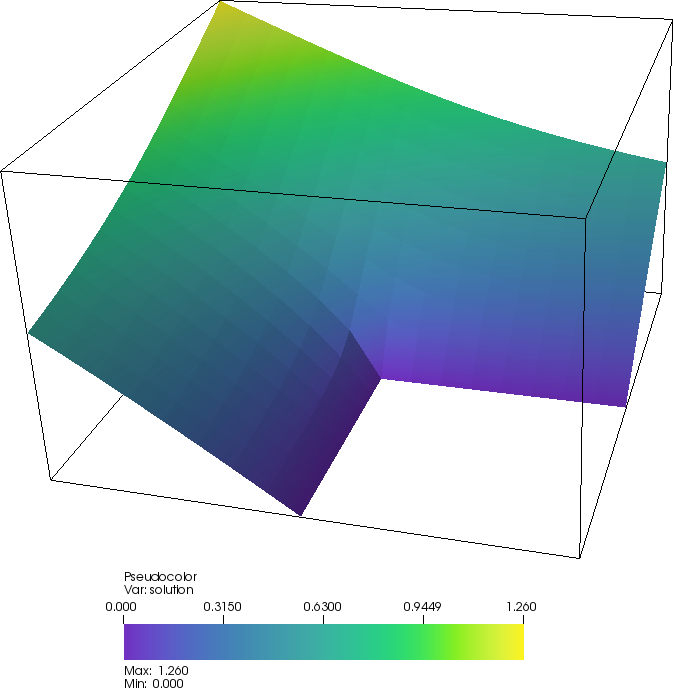
\includegraphics[width=0.5\textwidth]{figures/results/solution.png}
\caption{Solution of the manufactured Laplace problem on a L-shaped domain.}
\label{fig:solution}
\end{figure}

In this chapter, we will solve the so designed Laplace problem on the L-shaped domain on consecutively refined meshes, and evaluate certain aspects of our implementation, namely the error performance of the decision strategies and their parallel scalability.

Following the usual approach in \gls{fem}, we transfer our problem to its weak formulation using \gls{cg} methods:
\begin{align}
\left(\nabla u, \nabla v\right) &= 0 \,\text{,} & \forall v \in V &\coloneqq \left\{ v \in H^1(\Omega): v|_{\partial\Omega} = 0 \right\} \,\text{.}
\end{align}
The shape functions of Lagrangian elements will form the basis for the function space $V$. Dirichlet boundary conditions are imposed via constraints on \glspl{dof} located on boundaries. The problem will be solved numerically with an iterative solver based on the conjugate gradient algorithm combined with an \gls{amg} preconditioner.

The \dealii{} library offers interfaces to parallel linear algebra of the third party libraries \petsc{} \textcite{petsc3124} and \trilinos{} \textcite{trilinos12181} for distributed memory architectures. In our investigations, we choose the latter using their \epetra{}
%\textcite{epetra}
module that handles all data infrastructure, and pick a corresponding solver from their \aztecoo{}
%\textcite{aztecoo}
package as well as their \ml{}
%\textcite{ml}
preconditioner. Compared to an equivalent configuration of \petsc{} modules, the \trilinos{} implementation yields more reproducible results using \gls{mpi} \parencite[FAQ]{petsc3124} and performs faster with higher order polynomials at more advanced refinement iterations according to our experience. For all calculations, we set a tolerance of $10^{-12}$ relative to the $l_2$-norm of the right hand side vector of the equation system.



\section{Error versus performance}
\label{sec:errorvsperformance}

%Global H1 error as measure
%\begin{align}
%\| e_{hp} \|_{H^1(\Omega)}^2 &= \sum\limits_K \| e_{hp} (\vec{x}) \|_{H^1(K)}^2 \\
%\| e_{hp} \|_{H^1(K)}^2 &= \int_K (|e_{hp}|^2 + |\nabla e_{hp}|^2) \differential{\vec{x}}
%\end{align}
%with error function $e_{hp} = u - u_{hp}$.

% setup of scenario

The main motivation of \hp-adaptive methods are their superior error convergence characteristics compared to the more common \h-adaptive ones provided that the solution is sufficiently regular. We will demonstrate their advantages on our presented scenario and use consecutively adapted meshes to illustrate their error performance in relation to their workload on the numerical example.

%Demonstrate adaptive algorithms , and how the error reduces with.
%compare error with the workload either measured in the number of \glspl{dof} or the actual wall time. % maybe later

The consecutively adapted meshes so created are by far not optimal for the problem, nor is finding such an optimal mesh subject of this dissertation. We are rather interested in comparing the performance and results of the decision algorithms presented in Sec.~\ref{sec:decision}, and whether they are capable of localizing regions with singularities, i.e.\@ the one at the point of origin for our numerical example. We will compare all types of adaptation at our disposal, i.e.\@ \h-, \p-, and \hp-adaptation. For the latter, we examine all three presented strategies in contrast, namely error prediction and smoothness estimation by either Legendre or Fourier coefficient decay.

After solving the linear equation system in each step and calculating the error on basis of the analytic solution according to \textcite{kelly1983}, we use the \textit{fixed-number} strategy to indicate adaptation: The 30\% fraction of all cells with the highest error will be flagged for refinement, and 3\% of those with the lowest error will be marked for coarsening. This allows us to compare the results of each adaptation type under the same conditions, since always the same amount of cells is going to be changed. The idea behind additional coarsening is motivated by the fact that we tend to refine too many cells with error estimators providing an upper bound for the error, or error indicators based on heuristics. We would like to correct this from a previous iteration by coarsening a small amount of cells. The combination of fractions of 30\% for refinement and 3\% for coarsening has become a reasonable choice for two-dimensional applications within the \dealii{} library.

%We will compared different refinement strategies. We will use \textit{fixed-fraction} adaptation so that every cell is refined. This allows us to compare the choices of all strategies since always the same amount of cells is taken into account. \todo{see slack text}

Further for \hp-adaptive strategies, we need to choose a decision strategy providing corresponding indicators that propose which type of adaptation we want to impose one each cell.
%
Again, we use the \textit{fixed-number} algorithm on all decision indicators. This allows us to compare the choices made by each strategy since always the same amount of cells is going to be changed in terms of both \h- and \p-adaptation, respectively.
%
As a first naive approach, we will impose the \h-variant on one half of all cells previously marked for adaptation, and the \p-variant on the other half.
%As a first naive approach, we choose between \h- and \p-adaptation fifty fifty among all cells that have been previously marked for adaptation.
%, based on the specified decision criterion.
As a second attempt, since we know that we have only one single localized and well-defined singularity in the domain, we are confident to make an educated guess and assign 90\% of flagged cells for \p- and the remaining 10\% for \h-adaptation. From here, we refer to the first approach if we call a decision strategy naive, and speak of the second if no such attribute was given.

To setup the numerical example, we start with a mesh consisting of three cells as the coarsest possible representation of our L-shaped domain, which will be globally refined five times to form the initial grid for all investigations in this section.

The error prediction strategy forms an exception since it requires a prepended initialization step. In this case, we will begin with four initial refinement steps, solve the equation system, and perform another global refinement so that we have the corresponding prediction available. Further for this strategy, control parameters are set to $\gamma_n = 1$, $\gamma_h = 1$, and $\gamma_p = \sqrt{0.4}$, which corresponds to the values used by \textcites{melenk2001}{mitchell2014}.

We use a collection of Lagrangian finite elements $Q_p$ with polynomial degrees $p \in [2,7]$ and skip linear elements due to our observation that the smoothness estimation algorithms perform poorly with those. All cells will be initially assigned with the lowest order element. In the case of sole \h-adaptation, all elements will be assigned to $Q_2$ elements. For pure \p-adaptation, we favor \p-adaptation to \h-adaptation as long as the finite element can be \p-adapted, i.e.\@ the current finite element is neither at the top nor the bottom of the hierarchy. We perform a total of twelve consecutive adaptation iterations, so twice as many as there are different finite elements.

All calculations in this section have been carried out on a desktop machine, using an Intel \todo{trademark} Core i7-4790 processor running at 3.6 GHz with 32 GB of memory \todo{si}. Although this is a quad-core processor offering a total of eight threads utilizing hypertreading, we will only use a single thread for our calculations, which is sufficient to determine both error and workload. We will deal with parallelization in later sections.


% results: error vs ndofs

Representatively, we will show the grid and distribution of finite elements after six adaptation cycles of the Legendre coefficient decay strategy with the educated guess approach in Fig.~\ref{fig:fedegrees}. All other meshes after equally many adaptation iterations from the other strategies are showcased in App.~\ref{app::strategies}.

We see that the Legendre strategy is able to locate the singularity in the center by preferring \h-adaptive refinement in this section, while using \p-adaptation in the other regions. This is also the case for all other strategies, naiive or not, as shown in App.~\ref{app::strategies}.

\begin{figure}
\centering
Insert distribution of finite elements for Legendre strategy after five iterations.
\caption{Distribution of finite elements after five iterations with the Legendre coefficient decay strategy.}
\label{fig:fedegrees}
\end{figure}

We will plot the $H_1$ error against the workload, which can be measured in two ways: Either with the number of \glspl{dof}, or the elapsed real time from start to end of our application, which we refer to as wall time. We begin with identifying the workload with the former and show corresponding results in Fig.~\ref{fig:errordofs}.

%We measure the workload in two different ways and present the results separately. First, with the number of \glspl{dof} for each individual iteration, and second, with the total wall time accumulated over the current and all previous iterations.

\begin{figure}
\begin{subfigure}{1\textwidth}
  \centering
  \begin{tikzpicture}
\begin{loglogaxis}[
  xlabel=Number of \glspl{dof},
  ylabel=H1 error]
\addplot table [y=H1 error, x=ndofs, col sep=comma] {data/error/h.csv};
\addplot table [y=H1 error, x=ndofs, col sep=comma] {data/error/p.csv};
\addplot table [y=H1 error, x=ndofs, col sep=comma] {data/error/hp-legendre.csv};
\addplot table [y=H1 error, x=ndofs, col sep=comma] {data/error/hp-fourier.csv};
\addplot table [y=H1 error, x=ndofs, col sep=comma] {data/error/hp-prediction.csv};
\addplot table [y=H1 error, x=ndofs, col sep=comma] {data/error/hp-legendre-naive.csv};
\addplot table [y=H1 error, x=ndofs, col sep=comma] {data/error/hp-fourier-naive.csv};
\addplot table [y=H1 error, x=ndofs, col sep=comma] {data/error/hp-prediction-naive.csv};
\end{loglogaxis}
\end{tikzpicture}
  \caption{Double logarithmic representation. The thick line corresponds to the reference Eq.~(\ref{eq:errorbound_ana}).}
  \label{fig:errordofsloglog}
\end{subfigure}
\begin{subfigure}{1\textwidth}
  \centering
  \begin{tikzpicture}
\begin{semilogyaxis}[
%  scale only axis,
  xlabel=Number of \glspl{dof},
  ylabel=H1 error,
  legend pos=outer north east]
%\addplot table [y=H1 error, x=ndofs, col sep=comma] {data/error/h.csv};
%\addlegendentry{\h};

\addplot table [y=H1 error, x=ndofs, col sep=comma, select coords between index={0}{5}] {data/error/p.csv};
\addlegendentry{\p};

\addplot table [y=H1 error, x=ndofs, col sep=comma, select coords between index={0}{5}] {data/error/hp-legendre.csv};
\addlegendentry{\hp{}-Legendre};

\addplot table [y=H1 error, x=ndofs, col sep=comma, select coords between index={0}{5}] {data/error/hp-fourier.csv};
\addlegendentry{\hp{}-Fourier};

\addplot table [y=H1 error, x=ndofs, col sep=comma, select coords between index={0}{6}] {data/error/hp-prediction.csv};
\addlegendentry{\hp{}-prediction};

%\addplot table [y=H1 error, x=ndofs, col sep=comma] {data/error/hp-legendre-naive.csv};
%\addlegendentry{\hp{}-Legendre naive};
%
%\addplot table [y=H1 error, x=ndofs, col sep=comma] {data/error/hp-fourier-naive.csv};
%\addlegendentry{\hp{}-Fourier naive};
%
%\addplot table [y=H1 error, x=ndofs, col sep=comma] {data/error/hp-prediction-naive.csv};
%\addlegendentry{\hp{}-prediction naive};

%\addplot[very thick, samples=100, domain=10000:50000] {10^(-2)*exp(10^(-3.9)*(-x+10000))}; % {10^(-4)*(-x+10000)};
\end{semilogyaxis}
\end{tikzpicture}
  \caption{Customly scaled coordinate system with the y-axis scaled exponentially and the x-axis scaled with the cubic root. The thick line corresponds to the reference Eq.~(\ref{eq:errorbound_exp}) with $b = 0.18$.}
  \label{fig:errordofscustom}
\end{subfigure}
\caption{Error vs workload.}
\label{fig:errordofs}
\end{figure}

The double logarithmic representation of our results in Fig.~\ref{fig:errordofsloglog} reveals analytic convergence for the \h-adaptive case, but at a lower rate as presented in Eq.~(\ref{eq:errorbound_ana}), which translates to $n_\text{dofs}^{-1}$ in our scenario. An explanation would be that we are not working with quasiuniform but rather highly adapted meshes.

Eq.~(\ref{eq:errorbound_exp}) predicts exponential decay for \hp-adaptive strategies, which we would like to verify in Fig.~\ref{fig:errordofscustom} with a customly scaled plot featuring a logarithmic y-axis and an x-axis scaled with the cubic root, which corresponds to the correct exponent in our numerical example. Indeed, we see exponential convergence in the \p-adaptive and \hp-adaptive strategies to the proclaimed rate, however the naive approaches miss it. Thus a high proportion of \p-refinement is required to yield exponential decay in this scenario.

The \p-strategy shows a similar decay as the \hp-adaptive methods.%, but the error in the last cycle is still by a factor of two higher.
In this strategy, \p-refinement will be applied up to the point until it is no longer possible after we reached the highest order element in the hierarchy. With six distinct finite elements in our collection, we will apply \h-refinement for the first time after the sixth data point, at which a major drop is observable. We also see that the exponential decay proclaimed in Eq.~(\ref{eq:errorbound_exp}) is only observable after applying \h-refinement. Thus, we conclude that \h-refinement is mandatory to reduce the error to the observed low order of magnitude.

To solve the equation system in the last adaptation cycle, the \hp-adaptive methods %corresponding to our educated guess 
srequire a number of \glspl{dof} by a factor of 100 less than the \h-adaptive methods to reach the same accuracy
%need a factor of 1,000 less \gls{dof} to reach the same accuracy as the \h-adaptive methods
and by factor of 10 less compared to their naive counterparts. This demonstrates that \hp-adaptive methods are the methods of choice for this particular scenario.

%We conclude that \p-heavy refinement combined with \h-adaptation near the singularity perform the best error per workload ratio.

In the course of adaptation with the Fourier strategy, some adaptation steps increase the number of \gls{dof} without decreasing the error, which we refer to as 'hickups'.
%We see certain outliers in the plots for Fourier strategy.
We observed that they occur if the finite element with the highest polynomial degree in our mesh increases from fourth to fifth order. This is perhaps not a causal relation, and we have not yet found the reason for these 'hickups'.

%Compared to \h- and naive \hp-approaches, \p- and \hp-strategies featuring the educated guess yield similar results.

%We reach about one order of magnitude lower errors with \hp-adaptive strategies compared to the \p-adaptive, which might be due to the singularity that the latter does not resolve \todo{?}.


% results: error vs walltime

From a practical point of view, the error performance will now be compared to the actual wall time to measure whether we have an economic benefit in using \hp-adaptive methods. For each consecutive adaptation cycle, we again plot the calculated error against the workload, which is this time represented by the total run time accumulated over the current and all previous iterations. Each run will be repeated five times and the minimum over the total runtime over all runs will be picked to compensate for temporarily high loads on memory bandwidth. The results are shown in Fig.~\ref{fig:errorwalltime}.

\begin{figure}
%\begin{subfigure}{1\textwidth}
\centering
\begin{tikzpicture}
\begin{loglogaxis}[
  xlabel=Wall time {[seconds]},
  ylabel=H1 error,
  legend pos=outer north east]
\addplot table [y=H1 error, x=walltime, col sep=comma] {data/error/h.csv};
\addlegendentry{\h};

\addplot table [y=H1 error, x=walltime, col sep=comma] {data/error/p.csv};
\addlegendentry{\p};

\addplot table [y=H1 error, x=walltime, col sep=comma] {data/error/hp-legendre.csv};
\addlegendentry{\hp{}-Legendre};

\addplot table [y=H1 error, x=walltime, col sep=comma] {data/error/hp-fourier.csv};
\addlegendentry{\hp{}-Fourier};

\addplot table [y=H1 error, x=walltime, col sep=comma] {data/error/hp-prediction.csv};
\addlegendentry{\hp{}-prediction};

\addplot table [y=H1 error, x=walltime, col sep=comma] {data/error/hp-legendre-naive.csv};
\addlegendentry{\hp{}-Legendre naive};

\addplot table [y=H1 error, x=walltime, col sep=comma] {data/error/hp-fourier-naive.csv};
\addlegendentry{\hp{}-Fourier naive};

\addplot table [y=H1 error, x=walltime, col sep=comma] {data/error/hp-prediction-naive.csv};
\addlegendentry{\hp{}-prediction naive};
\end{loglogaxis}
\end{tikzpicture}
%  \caption{Error vs workload.}
%  \label{fig:errorexpworkload}
%\end{subfigure}
%\begin{subfigure}{1\textwidth}
%  \centering
%  \begin{tikzpicture}
\begin{semilogyaxis}[
  xlabel=Wall time {[seconds]},
  ylabel=H1 error,
  legend pos=outer north east]
%\addplot table [y=H1 error, x=walltime, col sep=comma] {data/error/h.csv};
%\addlegendentry{\h};

\addplot table [y=H1 error, x=walltime, col sep=comma, select coords between index={0}{5}] {data/error/p.csv};
\addlegendentry{\p};

\addplot table [y=H1 error, x=walltime, col sep=comma, select coords between index={0}{5}] {data/error/hp-legendre.csv};
\addlegendentry{\hp{}-Legendre};

\addplot table [y=H1 error, x=walltime, col sep=comma, select coords between index={0}{5}] {data/error/hp-fourier.csv};
\addlegendentry{\hp{}-Fourier};

\addplot table [y=H1 error, x=walltime, col sep=comma, select coords between index={0}{6}] {data/error/hp-prediction.csv};
\addlegendentry{\hp{}-prediction};

%\addplot table [y=H1 error, x=walltime, col sep=comma] {data/error/hp-legendre-naive.csv};
%\addlegendentry{\hp{}-Legendre naive};
%
%\addplot table [y=H1 error, x=walltime, col sep=comma] {data/error/hp-fourier-naive.csv};
%\addlegendentry{\hp{}-Fourier naive};
%
%\addplot table [y=H1 error, x=walltime, col sep=comma] {data/error/hp-prediction-naive.csv};
%\addlegendentry{\hp{}-prediction naive};

%\addplot[very thick, samples=100, domain=0.1:5] {10^(-2)*exp(10^(0)*(-x+0.1))}; % {10^(-4)*(-x+10000)};
\end{semilogyaxis}
\end{tikzpicture}
%  \caption{Error vs walltime.}
%  \label{fig:errorexpwalltime}
%\end{subfigure}
\caption{Double lagarithmic error vs walltime.}
\label{fig:errorwalltime}
\end{figure}

%We notice that the choice of the \hp-adaptive strategy has an impact on the error performance compared to the number of \glspl{dof}. However in comparing error with the runtime, we see that all methods perform similarly. We will postpone the discussion on this topic for the later Sec.~() in which we give an in-depth analysis on the sacalability of certain parts of our code, in which we think to identify the reason for this behavior.

Again after the last adaptation cycle, \p- and \hp-adaptive methods are most efficient and about an order of magnitude faster than the \h-adaptive variant. Interestingly, the wall times of the naive \hp-strategies fan out. It appears that a high diversity of finite elements compared with major grid adaptation increase the wall time significantly, and we suspect that the combination of solver and \gls{amg} preconditioner is responsible for this behavior. We will discuss this topic later in the scalability analysis.

The Fourier strategy takes the longest wall time for initialization, during which the Fourier transformation matrices are calculated. This is a costly operation, which requires substantially more quadrature points during calculation than the Legendre equivalent, and is responsible for the observable offset.

% this is general observation
Among all \hp-strategies of either naive or educated guess category, we do not see major differences in their performance, but overall the Legendre coefficient decay strategy stands out in both categories with the best error per workload performance in either way workload is defined.
%Compared to the Fourier strategy, it seems to be better suited for \gls{fem} since its basis functions are also based on polynomials.

% write this in the next chaper
%In the upcoming scalability analysis, we will thus pick this strategy with Legendre coefficient and the educated guess.

%Overall, the Legendre coefficient strategy yields the best error per workload performance in both categories.

%Again, to mitigate the impact of temporary slowdowns on the supercomputer due to a high loads on memory and network bandwidth, we repeat each run for a total of \todo{five?} times and take the minimal runtime in each category over all runs.
\section{Load balancing heuristics}
\label{sec:heuristics}

% introduction

For parallel computations on distributed memory systems, the global domain is partitioned into several subdomains, each of which is assigned to a single process. Such a mesh decomposition is showcased in Fig.~\ref{fig:decomposition}.

\begin{figure}
\centering
\begin{subfigure}[t]{.49\textwidth}
  \centering
  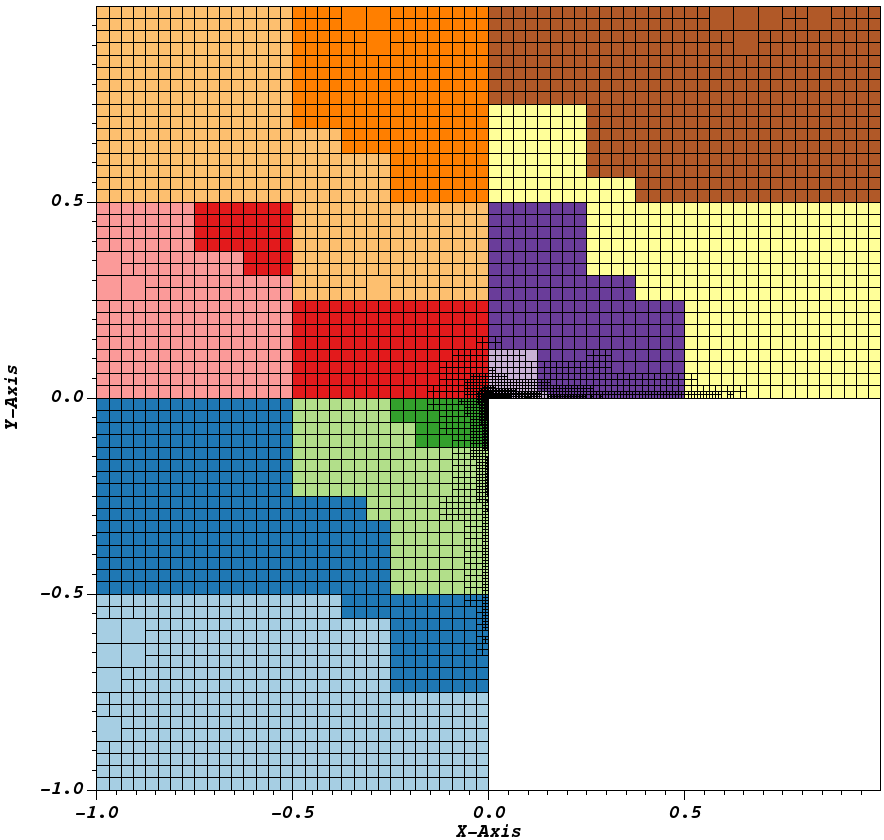
\includegraphics[width=\textwidth]{figures/results/corner-2d-error-hp-legendre-05_subdomain12.png}
  \caption{Constant weighting.}
\end{subfigure}
\begin{subfigure}[t]{.49\textwidth}
  \centering
  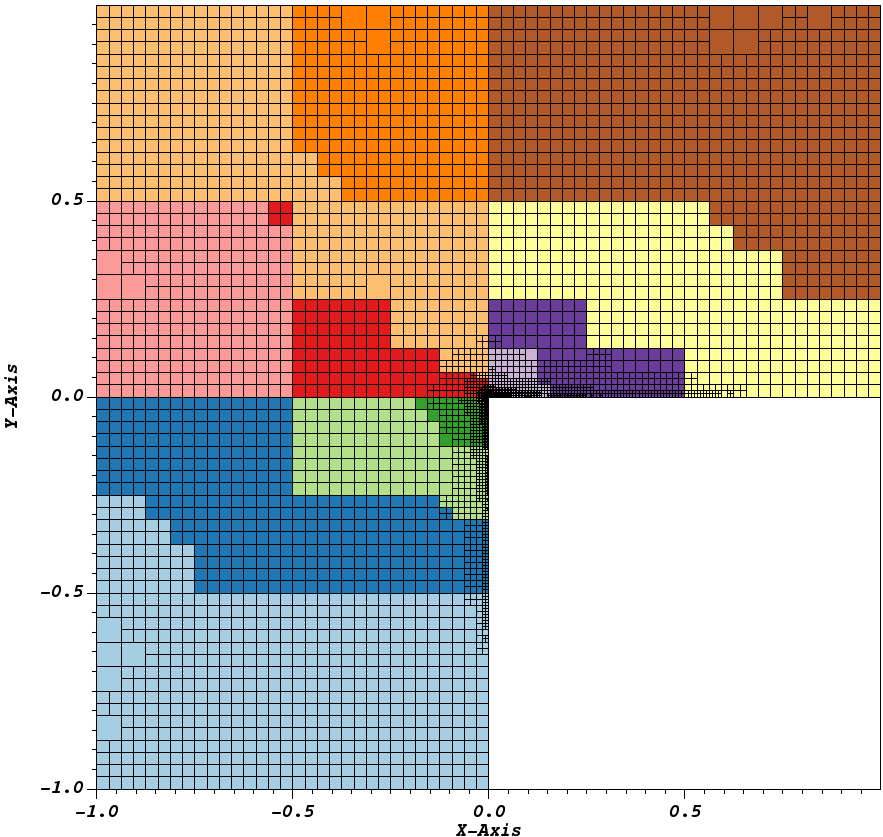
\includegraphics[width=\textwidth]{figures/results/corner-2d-error-hp-legendre-05_subdomain12_customweighting.png}
  \caption{Weighting with an individually potentiated number of \glspl{dof}, i.e.\@ $\propto n_\text{dofs}^{1.9}$.}
\end{subfigure}
\caption{Decomposition of the mesh after six iterations with the Legendre coefficient decay strategy on 12 \gls{mpi} processes with various cell weighting. Each color represents a different subdomain.}
\label{fig:decomposition}
\end{figure}

Proper load balancing is necessary for an efficient use of all computational resources. Especially on \gls{hpc} systems with lots of available processors, this is a critical feature. For \hp-adaptive \gls{fem}, we presented approaches for load balancing in Sec.~\ref{sec:loadbalancing} by assigning weights to each individual cell and balancing the accumulated weight among all processes. We relate the weight to the number of \glspl{dof} on each cell potentiated by an exponent that we will determine in the upcoming investigations. Or in other words, cell weights are chosen proportional to $n_\text{dofs}^c$ with the exponent $c$ to be ascertained.

Although all three \hp-adaptive strategies have demonstrated a similar performance as shown in Sec.~\ref{sec:errorvsperformance}, we pick only one adaptation strategy for our parallel investigations. We choose the smoothness estimation strategy based on the decay of Legendre coefficients as the most efficient one for this purpose.

% system specifications

Investigations are carried out on the JURECA supercomputer \parencite{krause2016}. Each computing node is equipped with two Intel\textsuperscript{\textregistered} Xeon\textsuperscript{\textregistered} E5-2680 v3 processors with twelve cores running at 2.5GHz and either 128GB, 256GB or 512GB of memory. With simultaneous multithreading, a total of 48 threads are available per node. Communication between nodes happens via a Mellanox EDR InfiniBand high-speed network.

In this section, our investigations are performed on two distinct nodes, which provide a total of 96 threads and involve communication between two physically independent memory segments. We expect that this setup yields representative results that can be extrapolated on even larger problem sizes.

Further, we use a 'flat' \gls{mpi} model: Every thread will be assigned to an individual \gls{mpi} process and no additional thread parallelization is invoked. Although \dealii{} provides such a feature via Intel\textsuperscript{\textregistered} \gls{tbb}, we refrain from using it to measure the pure \gls{mpi} performance for all parallel analyses in this dissertation.

% problem specifications

To qualify our problem for parallel computations, we need to increase its size drastically. The problem is initialized with nine global refinements and gets adapted in twelve iterations. For the strategy with the Legendre coefficient decay, this results in a total number of 46,369,440 \glspl{dof}, so that in the best case each process will be assigned to a number of 483,015 \glspl{dof} on average. Each type of finite element from the provided collection is represented at least once in the mesh.

This advanced scenario will form the basis of our investigations to see how different weighting exponents affect the wall time, and which one provides a minimum. With serialization, we ensure that each of these runs conforms to the same conditions. Again, to mitigate the impact of temporary slowdowns on the supercomputer due to high loads on memory and network bandwidth, we repeat each run for a total of five times and take the minimum wall time in each category over all runs.

% results

For varying weighting exponents, we compare the wall times of the full adaptation cycle and its relevant sections
%For resumed scenarios in which the mesh will be partitioned according to weights with different weighting exponents, we compare the wall time of critical sections of the program as well as the total wall time
%between runs with different weighting exponents
in Fig.~\ref{fig:weights}.

\todo{Second scale for assembly/discontinued axis with groupplot}
%https://tex.stackexchange.com/questions/46422/axis-break-in-pgfplots
\todo{Maybe also add setup of data structure and other parts}
\begin{figure}
\centering
\begin{tikzpicture}
\begin{axis}[
  xlabel=Weighting exponent,
  ylabel=Wall time {[seconds]},
  legend pos=outer north east]

\addplot table [y=full cycle, x=weighting exponent, col sep=comma] {data/weight/weight.csv};
\addlegendentry{full cycle};

\addplot table [y=assembly, x=weighting exponent, col sep=comma] {data/weight/weight.csv};
\addlegendentry{assemble linear system};

\addplot table [y=solve, x=weighting exponent, col sep=comma] {data/weight/weight.csv};
\addlegendentry{linear solver and preconditioner};
\end{axis}
\end{tikzpicture}
\caption[Wall times for load balancing with varying weighting exponents.]{Wall times of a complete adaptation cycle and those parts relevant for load balancing. The problem has a number of about 46 million \glspl{dof} and is solved on 2 nodes or 96 \gls{mpi} processes. Weights proportional to $n_\text{dofs}^c$ will be assigned to each cell with varying exponents $c$.}
\label{fig:weights}
\end{figure}

As discussed in Sec.~\ref{sec:balancing}, the assembly of the equation system and the its solution are identified as the critical sections whose wall time is affected by the number of \glspl{dof}. We see that the solution of the equation system takes about 90\% of the total wall time and is the crucial factor for proper load balancing. The minimal wall time for both solver and the full cycle is reached with a weighting exponent of $c = 1.9$.

We were surprised to find the minimum wall time of the solver at such a high exponent, since we expected $c = 1$ for an efficient solver. This may be related to the implementation of the preconditioner combined with the disorder that \hp-adaptive methods cause in the system matrix. Further, we were expecting a minimum in the assembly at about $c = 2$, but found it was decaying at even higher exponents. We have no explanation for this behavior. Analyzing the effect of cell weighting on each individual section of the program
%the load balancing
will be subject of further investigations.

% Next step
%We set an weighting expoenent to a value of $c = 1.9$ for the following considerations regarding scalability.

\section{\Glsfmtlong{hpc} scalability}
\label{sec:scaling}

The final part of our investigations relates to the demonstration of the scalability of our algorithms and data structures on \gls{hpc} systems, for which we will again use the JURECA supercomputer \parencite{krause2016}.

Again working with successively adapted meshes, we will measure the wall time spent in each particular section of each SOLVE-ESTIMATE-MARK-REFINE iteration, which is supposed to increase linearly with the workload determined by the number of \glspl{dof} or decrease linearly with an increasing amount of workers, i.e.\@ number of \gls{mpi} processes. We distinguish between the following categories in each adaptation cycle similar to \textcite{bangerth2012}:
\begin{itemize}
\item \textit{Setup data structures}. Enumerate all \glspl{dof}. Determine the sparsity pattern describing locations of nonzero matrix entries. Calculate constraints for hanging nodes and boundary values. Allocate memory for all distributed data structures. Communicate between processes which matrix or vector elements they will write to that they do not own locally.
\item \textit{Assemble linear system}. Calculate the individual contribution of each locally owned cell to the global equation system. Exchange data if matrix or vector elements are stored on a different process.
\item \textit{Linear solver and preconditioner}. Setup both the \gls{amg} preconditioner and the conjugate gradient solver and solve the equation system in parallel.
\item \textit{Estimate error}. Calculate the error indicators on locally owned cells on basis of the current solution. Mark cells for either refinement or coarsening by computing global thresholds.
\item \textit{Estimate smoothness}. Calculate the smoothness indicators on basis of the current solution on locally owned cells marked for either refinement or coarsening. Decide whether \h- or \p-adaptation is going to be applied by computing global thresholds.
\item \textit{Coarsen and refine}. Perform coarsening and refinement and maintain the 2:1 cell balance on the \pforest{} master mesh, followed by its repartitioning. Transfer data between the outdated and updated mesh. Apply all changes made to the master mesh on the \dealii{} triangulation.
\end{itemize}

We will pick the parameters and features that have proven to be suitable in our numerical example. Thus, we again choose smoothness estimation by the decay of Legendre coefficients as our \hp-decision strategy. For load balancing, cell weighting is imposed proportional to the number of \glspl{dof} on each cell potentiated by the exponent $c = 1.9$.


% weak scaling

For weak scaling, problems with increasing size are solved on a fixed number of \glspl{mpi} processes, which we will realize using consecutive adaptations. We choose two different numbers of computation nodes, namely 16 and 64 nodes with 768 and 3,072 \glspl{mpi} processes in total each.

We initialize the problem with ten initial global refinements and adapt the mesh for a total of 11 iterations with the smaller amount of computing nodes, and 12 iterations for the larger one. In the chosen configuration, all available memory is used on the assigned nodes, so no more adaptation cycles are possible without running out of memory. Again to exclude the influence of the current load on the supercomputer, all runs are performed multiple times and the minimum wall time of each category is taken. This time we repeat each run seven times. The results of weak scaling are shown in Fig.~\ref{fig:weak} up to problem sizes of 2,073,075,769 \glspl{dof}.

\begin{figure}
\begin{subfigure}{1\textwidth}
  \centering
  \begin{tikzpicture}
\begin{loglogaxis}[
  xlabel=Number of \glspl{dof},
  ylabel=Wall time {[seconds]},
  legend pos=outer north east]

% data
\addplot table [y=solve, x=ndofs, col sep=comma] {data/weak/weak-nodes16.csv};
\addlegendentry{linear solver and preconditioner};

\addplot table [y=setup, x=ndofs, col sep=comma] {data/weak/weak-nodes16.csv};
\addlegendentry{setup data structures};

\addplot table [y=assembly, x=ndofs, col sep=comma] {data/weak/weak-nodes16.csv};
\addlegendentry{assemble linear system};

\addplot table [y=compute errors, x=ndofs, col sep=comma] {data/weak/weak-nodes16.csv};
\addlegendentry{estimate error};

\addplot table [y=calculate indicators, x=ndofs, col sep=comma] {data/weak/weak-nodes16.csv};
\addlegendentry{estimate smoothness};

\addplot table [y=refine, x=ndofs, col sep=comma] {data/weak/weak-nodes16.csv};
\addlegendentry{coarsen and refine};

% optimal line
\addplot[very thick, samples=2, domain=12591105:1302365268] {10^(-7.2)*x};
\addlegendentry{optimal convergence};

% auxiliary lines
\begin{scope}
  \draw[green] ({axis cs:76800000,0}|-{rel axis cs:0,1}) -- ({axis cs:76800000,0}|-{rel axis cs:0,0});
  \draw[blue] ({axis cs:50647318,0}|-{rel axis cs:0,1}) -- ({axis cs:50647318,0}|-{rel axis cs:0,0});
\end{scope}
\addlegendimage{color=green};
\addlegendentry{$10^5$ \glspl{dof} per process};
\addlegendimage{color=blue};
\addlegendentry{each finite element in mesh};
\end{loglogaxis}
\end{tikzpicture}%
  \caption{Weak scaling on 16 nodes or 768 \gls{mpi} processes.}
  \label{fig:weak-nodes16}
\end{subfigure}
\begin{subfigure}{1\textwidth}
  \centering
  \begin{tikzpicture}
\begin{loglogaxis}[
  xlabel=Number of \glspl{dof},
  ylabel=Walltime {[seconds]}]

\addplot table [y=full cycle, x=ndofs, col sep=comma] {data/weak/weak-nodes64.csv};

\addplot[very thick, samples=2, domain=12591105:2073075769] {10^(-3)*x};

\end{loglogaxis}
\end{tikzpicture}%
  \caption{Weak scaling on 64 nodes or 3,072 \gls{mpi} processes.}
  \label{fig:weak-nodes64}
\end{subfigure}
\caption{Weak scaling for consecutively refined meshes on different numbers of \glspl{mpi} processes. Each \gls{mpi} process has more than $10^5$ \glspl{dof} assigned only to the right side of the indicated vertical line. Each finite element is represented at least once in the mesh only to the right side of the designated vertical line.}
\label{fig:weak}
\end{figure}

\textcite{bangerth2012} proclaimed that linear scaling is observable in all categories if the number of \glspl{dof} per \gls{mpi} process exceeds $10^5$. We can confirm this observation in our numerical example with parallel \hp-adaptation as well.

During the first few adaptation cycles in our application, the wall time attributed to the solution category shows a major increase which is much more than just linear. After six adaptation cycles, i.e.\@ right of the indicated vertical line in Fig.~\ref{fig:weak}, each finite element will be represented at least once in the domain due to the way we configured the scenario, and the aforementioned curve flattens and increases only linearly as expected.

%We suspect that the randomness of the distribution of 

%We suspect that the mixture of many different finite elements are the reason for this behavior

%that adding finite elements of a higher order than before results in a higher complexity in the matrix, that is responsible for a longer solution.
We suspect that the rather heterogeneous allocation of the finite elements by the decision algorithms
%has a negative influence on the conditioning of the system matrix and
has a similar effect on the distribution of nonzero entries in the system matrix, for which \gls{amg} preconditioners are not designed for. It appears that we could make use of a more suitable preconditioner. Although it was the best option at our disposal at the time this dissertation was written, we may think about an alternative to this for future applications. Instead of relying on \gls{amg} methods, \gls{gmg} preconditioners are expected to work more robust and should be the method of choice.

\Gls{gmg} methods for \hp-adaptive refinement in serial applications have already been developed by \textcite{mitchell2010}. \textcite{clevenger2019} worked out \gls{gmg} preconditioners for parallel \h-adaptive \gls{fem} and made their algorithm available in the \dealii{} library. The development of a corresponding preconditioner for parallel \hp-adaptive \gls{fem} will be subject of future work, as well as its application and comparison with the \gls{amg} equivalents.


% strong scaling

For strong scaling, problems are set to a fixed size and being solved with a increasing amount of \gls{mpi} processes. This time, we just solve one individual adaptation cycle on a tailored mesh, that has been prepared from a previous run via serialization.
%, we prepare a tailored mesh for these considerations, and solve that particular cycle with a varying number of processors.

To prepare these meshes, we consider two different scenarios which will be constructed as follows: A smaller scenario is initialized with ten global refinements, and a larger one with twelve refinements. Both will be adapted successively in six adaptation cycles, which results in each finite element being represented at least once in the whole domain. This leads to number of \glspl{dof} of 50,736,415 and 969,257,276 in total for the respective scenario.

With serialization, both problems will be solved at their advanced stage with varying amounts of \gls{mpi} processes, and the wall times of each section in the program will be recorded. We again repeat each run for a total of seven times and take the minimum wall time in each category, except for the largest run in order to solve the bigger problem on 1,024 nodes or 49,152 \gls{mpi} processes, which we could only repeat five times before we completely exhausted our entire computing time quota. The results of strong scaling are shown in Fig.~\ref{fig:strong}.

\begin{figure}
\begin{subfigure}{1\textwidth}
  \centering
  \begin{tikzpicture}
\begin{loglogaxis}[
  xlabel=Number of \gls{mpi} processes,
  ylabel=Walltime {[seconds]}]

\addplot table [y=full cycle, x=ncpus, col sep=comma] {data/strong/strong-nrefs10_withoutlarge.csv};

\addplot[very thick, samples=2, domain=48:6144] {10^(3)*x^(-1)};

\end{loglogaxis}
\end{tikzpicture}%
  \caption{Strong scaling for a fixed problem size of roughly 51 million \glspl{dof}.}
  \label{fig:strong-nrefs10}
\end{subfigure}
\begin{subfigure}{1\textwidth}
  \centering
  \begin{tikzpicture}
\begin{loglogaxis}[
  xlabel=Number of \gls{mpi} processes,
  ylabel=Wall time {[seconds]},
  legend pos=outer north east]

% data
\addplot table [y=solve, x=ncpus, col sep=comma] {data/strong/strong-nrefs12.csv};
\addlegendentry{linear solver and preconditioner};

\addplot table [y=setup, x=ncpus, col sep=comma] {data/strong/strong-nrefs12.csv};
\addlegendentry{setup data structures};

\addplot table [y=assembly, x=ncpus, col sep=comma] {data/strong/strong-nrefs12.csv};
\addlegendentry{assemble linear system};

\addplot table [y=compute errors, x=ncpus, col sep=comma] {data/strong/strong-nrefs12.csv};
\addlegendentry{estimate error};

\addplot table [y=calculate indicators, x=ncpus, col sep=comma] {data/strong/strong-nrefs12.csv};
\addlegendentry{estimate smoothness};

\addplot table [y=refine, x=ncpus, col sep=comma] {data/strong/strong-nrefs12.csv};
\addlegendentry{coarsen and refine};

% optimal line
\addplot[very thick, samples=2, domain=768:49152] {10^(5)*x^(-1)};
\addlegendentry{optimal convergence};

% auxiliary lines
\begin{scope}
  \draw[green] ({axis cs:9692.57276,0}|-{rel axis cs:0,1}) -- ({axis cs:9692.57276,0}|-{rel axis cs:0,0});
\end{scope}
\addlegendimage{color=green};
\addlegendentry{$10^5$ \glspl{dof} per process};
\end{loglogaxis}
\end{tikzpicture}%
  \caption{Strong scaling for a fixed problem size of roughly 970 million \glspl{dof}.}
  \label{fig:strong-nrefs12}
\end{subfigure}
\caption{Strong scaling for one advanced adaptation cycle at different problem sizes. Each \gls{mpi} process has more than $10^5$ \glspl{dof} assigned only to the left side of the indicated vertical line.}
\label{fig:strong}
\end{figure}

Again, we identify linear scaling whenever the number of \glspl{dof} per \gls{mpi} process exceeds $10^5$, which again coincides with the observations of \textcite{bangerth2012}.
  \chapter{Summary and outlook}
\label{ch:summary}
\glsresetall

% summary

The \gls{fem} offers the unique capability of \hp-adaptive methods with remarkable properties in error convergence relative to workload. However for \gls{hpc}, their parallel implementation for large scale computing architectures with distributed memory via \gls{mpi} is difficult.

We presented generic algorithms and data structures for massively parallel \hp-adaptive \gls{fem}, which allow for dynamic changes in both grid resolution and assignment of finite elements. Our findings are independent of the implementation and can be used to enhance any kind of \gls{fem} software, provided that their concepts conform to the elementary work of \textcite{bangerth2009,bangerth2012}, which forms the basis of our research.

%can be enhanced with these findings, provided they already feature parallel \h-adaptive and sequential \hp-adaptive methods by \textcite{bangerth2009,bangerth2012}.

%provided that their underlying structure is compatible with 

%which can be used to enhance any existing \gls{fem} software. 

In this dissertation, we elaborated on the non-trivial parts of combining both parallel \h-adaptive and sequential \hp-adaptive methods.
%, which are briefly recapped in the following:
%\begin{itemize}
%\item%
The unique enumeration of \glspl{dof} and their affiliation with the owning \gls{mpi} process poses challenges for \gls{cg} methods whenever finite elements of similar or different polynomial degree meet on subdomain boundaries. We developed an algorithm for the unique enumeration of \glspl{dof} in the parallel \hp-adaptive context which does not require more costly communication with ghost cells than the \h-adaptive pendant.

%\item%
For an automatic adaptation, refinement criteria on basis of error indicators are required to decide which parts of the domain should be adapted. In addition using \hp-adaptive methods, we also have to select the type of adaptation we would like to impose.
%In addition to the determination of refinement criteria on basis of error indicators, we need to additionally decide which type of adaptation to impose for an automatic determination.
We presented several state-of-the-art methods for \hp-refinement, prepared them for parallel applications, and enhanced them for \hp-coarsening as well.
%\end{itemize}

%\item%
Cells are distributed on \gls{mpi} processes in such a way that the workload is balanced among them, which we ensure by a weighted repartitioning. On each cell, we imposed a simple weight proportional to the \glspl{dof} potentiated by a factor which depends on the problem to investigate.

%\item%
Whenever the mesh itself changes in parallel applications, for example by adaptation, workload needs to be redistributed by repartitioning. Depending on the investigated problem, transferring data from the former to the updated mesh is necessary, for example the finite element approximation itself. In addition using \hp-adaptive methods, the amount of data to be transferred might vary by cell. We present a general approach to provide contiguous memory sections which will be exchanged using optimized algorithms presented by \textcite{burstedde2018} for data of fixed and variable size, respectively.

%We use optimized algorithms presented by .

%Data transfer of variable size via \gls{mpi} and the necessity of contiguous memory chunks to easily address each processor's locally owned space.

We provided a reference implementation in the \dealii{} library and applied it to the Laplace problem on an L-shaped domain, a common numerical benchmark for \hp-adaptive methods. We have demonstrated their superior error convergence and shown that our implementation scales on up to 49,152 \gls{mpi} processes.

%While sequential, static \hp-adaptive methods have been frequently used in multi-physics problems in \dealii{}, the actual application of dynamic \hp-adaptive methods stayed mostly in an experimental state within \dealii{} because of its intricate application. With the current interface as redesigned in this dissertation hopefully simplifies its usage so that it attracts for users and it hopefully becomes a widely used feature in the community.


% extensions

Algorithms for parallel \hp-adaptive \glspl{fem} capable of handling both \gls{cg} and \gls{dg} methods have not yet been prepared in a general framework like this before. However, our implementation is still at an early stage of development, and there is still plenty of room for improvement, as we described throughout this dissertation. Those aspects that leave room for improvements are the following.

We observed an unfavorable scaling behavior during the solution of the equation system in our \hp-adaptive \gls{fem} application, which we attribute to our choice of \gls{amg} preconditioning. A preconditioner that also incorporates multilevel methods on a hierarchy of finite elements with different polynomial degrees $p$ will be more efficient and solve the linear equation system in less iterations as investigated by \textcite{mitchell2010}. They embedded \p-multigrid methods in \gls{gmg} preconditioning for sequential \hp-adpative applications. Furthermore, \textcite{fehn2019} combined multilevel methods on hierarchies in a polynomial, geometric, and algebraic sense for parallel \gls{fem} on static meshes without adaptation. Future work involves the combination of multilevel methods to make them available for parallel \hp-adaptive methods as well.
This also incorporates parallel \h-adaptive \gls{gmg} preconditioners that have been presented by \textcite{clevenger2019} who also provided an implementation in the \dealii{} library.
%for which \gls{gmg} methods are promising. For parallel \h-adaptive \gls{fem}, \textcite{clevenger2019} presented algorithms for \gls{gmg} preconditioners and provided an implementation in the \dealii{} library. Future work involves enhancing them for \hp-adaptive methods as well, combining their ideas with those of \textcite{mitchell2010}.

%Geometric multigrid
%Find a way to combine the parallel \h-adpative \gls{gmg} preconditioner by \textcite{clevenger2019} with the \hp-adaptive variant by \textcite{mitchell2010}.

%how to combine them with the ideas of melenk for \hp-adaptive \gls{gmg} methods.

%new strategies to decide between \h- and \p-adaptation
We described a handful of decision strategies to choose between types of adaptation. However, there are more strategies worth trying out.
%Regularity estimation (see houston 2005 for references), houston 2003
%\textcite{houston2003} \textcite{houston2005}
\textcite{houston2003,houston2005} directly determined the regularity of the solution from the coefficients of a Legendre expansion of the finite element approximation. We could use those as decision indicators, or directly set the fitting finite element on basis of their result.
%Enhancements for Fourier strategy using \gls{fft} (e.g. via \fftw{} \parencite{frigo2005,fftw338}).
%Further, we noticed that the preparation of the Fourier transformation matrices consumes a lot of wall time due to the larger number of quadrature points required for integration, which we hope to accelerate using \gls{fft}, for example via \fftw{} \parencite{frigo2005,fftw338}.

One could also imagine different decision indicators that are specific to the investigated problem. Hence for computational fluid dynamics, we could relate the decision criteria towards a measure for turbulence for example. The absolute value of the vorticity $\vec{w} = (\nabla \times \vec{v})$ as the rotation of the fluid velocity $\vec{v}$ would make up a good measure. We would prefer \h-refinement on turbulent regions indicated by a high vorticity, and \p-refinement in laminar regions.

%Let us consider for examples computational fluid dynamics. We could use different criteria to decide for \hp-adaptation. The vorticity $\vec{w} = (\nabla \times \vec{v})$ or the dimensionless Reynolds number $\mathrm{Re} = (v L / \nu)$ would make up a good measure, with the velocity $\vec{v}$, the kinematic viscosity $\nu$ and a characteristic length $L$. We would prefer \h-refinement on turbulent regions indicated by a high vorticity or Reynolds number, and \p-refinement in laminar regions.

Future work will involve examining the possibility to combine \hp-adaptive methods with so called matrix-free methods. Memory access is the current bottleneck on \gls{hpc} machines. Instead of calculating matrix entries and storing them, it might be faster to calculate them on the fly as they are requested. Combined with \gls{simd} instructions or \gls{gpu} acceleration, this is a highly favorable strategy on current \gls{hpc} machines. Matrix-free methods have been part of the \dealii{} for a long time \parencite{kronbichler2012}, and have been continuously enhanced during the last decade \parencite{kronbichler2019}. Furthermore, \textcite{munch2020} recently published an open-source library named \texttt{hyper.deal} using high-order \gls{dg} methods for high-dimensional partial differential equations, which is built on top of \dealii{} and provides an easy-to-use interface to utilize these methods. The purpose of their framework is to investigate the dynamics of plasmas in nuclear fusion reactors involving shocks, which are modeled using the six-dimensional Vlasov equation. An extension with \hp-adaptive methods would be highly promising in any case and would unleash their full potential. A specialized decision strategy for \hp-adaptation tied to an observable might be more suitable in the context of plasmas than the general strategies presented in this project.

More generally, this framework can also be used to solve many other problems in continuum mechanics as well, e.g., structural mechanics and fluid dynamics in general. As a concrete application example in geosciences, convection processes in Earth's mantle can be simulated with the open-source code \texttt{ASPECT} \parencite{kronbichler2012a,aspect210} which builds upon the \dealii{} library. Simulation on a domain of planetary scope yields a lot of workload. Thus \texttt{ASPECT} already benefits tremendously from parallel \h-adaptive methods, and now also has parallel \hp-adaptive methods at its disposal with the results of our project.


% closing words

We are left to see whether \hp-adaptive \gls{fem} for architectures with distributed memory will be well-received by the community. At the very least, it has been a long requested feature of the \dealii{} library, which was first mentioned in the \dealii{} Google group\footnote{\url{https://groups.google.com/d/msg/dealii/BmEF75lOA_E/PjyF9F5Uo3UJ}} in early 2014 and has been in progress since late 2016 \textcite{dealiiissue3511}.

In the past, \textcite{bangerth2009} provided algorithms and data structures for sequential \hp-adaptive methods and provided a reference implementation in \dealii{}. They have been widely used for multi-physics problems in \dealii{}, coupling different physical models in different parts of the domain by assigning corresponding finite elements. However, automatic \hp-adaptation stayed mostly in an experimental state within \dealii{} because of its intricate application. The current interface has been redesigned in this project and simplifies its usage, so that it hopefully becomes a widely used feature in the community.

A good approach to make these features more accessible to all users of the library is to write a dedicated tutorial program as part of the \dealii{} library that showcases the new functionality presented in this dissertation. Tutorial programs are meant to demonstrate certain features of the library and give newcomers a fundamental insight into the numerical and computational background, as well as into implementation details due to extensive documentation.
%The \dealii{} library currently features a total of 62 of such tutorial programs in their most recent release \parencite{arndt2019}.
For the demonstration of parallel \hp-adaptive \gls{fem}, we will translate the numerical example from Ch.~\ref{ch:results} into a new stand-alone tutorial as a next step.

% We are left to provide an easily accessible tutorial program describing all features in the tradition of the \dealii{} library.

%Time will tell how this feature is going to be perceived by the scientific community.

%It has been a long requested feature in the \dealii{} library, which was first mentioned in the \dealii{} Google group\footnote{\url{https://groups.google.com/forum/\#!forum/dealii}} in late 2015, and work began in late 2016 \textcite{dealiiissue3511}.

% has now finally been implemented in a way that it is easily accessible by made

%It was first requested by the community as a feature mentioned in late 2015 in the deal.
%The first mention in the \dealii{} Google group\footnote{\url{https://groups.google.com/forum/\#!forum/dealii}} happened in late 2015, and work began in late 2016 \textcite{dealiiissue3511}.

After all, parallel \hp-adaptive methods offer promising capabilities, and with all features left to add they are a very challenging yet exciting topic worth to continue working on.

%And if the scientific interest will be underwhelming, we can at least still create nice pictures with it.
  
  \appendix
  \chapter{Enumeration of \glsfmtlongpl{dof}: Demonstration}
\label{app::enumeration}

This section delivers the lengthy demonstration of the enumeration algorithm for \glspl{dof} on the corresponding benchmark from sec.\@ \ref{sec:enumeration}.

The test case is composed out of four adjacent cells, from which two catty-cornered ones are assigned to the same Lagrangian finite element of either order two or four. The mesh is divided into two subdomains, each containing two neighboring cells of different finite element. The setup of the benchmark is shown in fig.\@ \ref{fig:enumdemosetup}.

We apply the algorithm step-by-step on this particular example and present its intermediate states in fig.\@ \ref{fig:enumdemosteps}.

\todo{Add benchmark test figure.}
\begin{figure}
  \centering
  \caption{Test setup for the enumeration algorithm for \glspl{dof}.}
  \label{fig:enumdemosetup}
\end{figure}

\todo{Add step-by-step figures.}
\begin{figure}
  \centering
  \caption{Step-by-step demonstration of the enumeration algorithm for \glspl{dof} on the test case. Changes made at each step are highlighted.}
  \label{fig:enumdemosteps}
\end{figure}
  \chapter{Comparison of decision strategies for \hp-adaptation}
\label{app::strategies}
\glsresetall

In this section, we oppose the adaptation behavior of all utilized strategies applied on our numerical example from Sec.~\ref{sec:errorvsperformance}, i.e., \h-, \p-, and \hp-adaptation with corresponding decision strategies of error prediction and smoothness estimation by the decay of Fourier and Legendre coefficients.

We depict the distribution of finite elements after six consecutive adaptation steps, in which \SI{30}{\percent} of cells with the highest error will be refined, and \SI{3}{\percent} will be coarsened. For \hp-adaptation, half of all those cells will be flagged for \h- and \p-adaptation as a naive approach. In a second attempt, \SI{90}{\percent} of cells marked for adaptation will be flagged for \p-adaptation, while the remaining \SI{10}{\percent} will be \h-adapted. We call the second approach an educated guess for our numerical example.

The meshes of pure \h- and \p-adaptation are shown in Figs.~\ref{fig:meshh},~\ref{fig:meshp}. For each \hp-adaptation strategy, grids generated with either the naive or educated guess approach are depicted in Figs.~\ref{fig:meshfourier},~\ref{fig:meshlegendre},~\ref{fig:meshprediction}.


\begin{figure}
\centering
\begin{tikzpicture}
\begin{axis}[
  scale=1.3,
  xmin=-1,xmax=1,
  ymin=-1,ymax=1,
  unit vector ratio={1 1},
  tick align=outside,
  xlabel=$x$,
  ylabel=$y$,
  colormap/OrRd,
  colorbar sampled,
  colorbar style={ylabel={finite element polynomial degree}, samples=7},
  point meta min=1.5,
  point meta max=7.5
]

\addplot graphics [
  xmin=-1,xmax=1,
  ymin=-1,ymax=1,
] {figures/appendix/strategies/corner-2d-errors-h-05.pdf};
\end{axis}
\end{tikzpicture}
\caption[Arrangement of finite elements with \h-adaptation.]{Arrangement of finite elements after six adaptation iterations with \h-adaptation. The colors represent different polynomial degrees $p$ of the assigned Lagrange elements $Q_p$.}
\label{fig:meshh}
\end{figure}

\begin{figure}
\centering
\begin{tikzpicture}
\begin{axis}[
  scale=1.3,
  xmin=-1,xmax=1,
  ymin=-1,ymax=1,
  unit vector ratio={1 1},
  tick align=outside,
  xlabel=$x$,
  ylabel=$y$,
  colormap/OrRd,
  colorbar sampled,
  colorbar style={ylabel={finite element polynomial degree}, samples=7},
  point meta min=1.5,
  point meta max=7.5
]

\addplot graphics [
  xmin=-1,xmax=1,
  ymin=-1,ymax=1,
] {figures/appendix/strategies/corner-2d-errors-p-05.pdf};
\end{axis}
\end{tikzpicture}
\caption[Arrangement of finite elements with \p-adaptation.]{Arrangement of finite elements after six adaptation iterations with \p-adaptation. The colors represent different polynomial degrees $p$ of the assigned Lagrange elements $Q_p$.}
\label{fig:meshp}
\end{figure}

\begin{figure}
\begin{subfigure}{1\textwidth}
  \centering
  \begin{tikzpicture}
\begin{axis}[
  scale=1.3,
  xmin=-1,xmax=1,
  ymin=-1,ymax=1,
  unit vector ratio={1 1},
  tick align=outside,
  xlabel=$x$,
  ylabel=$y$,
  colormap/OrRd,
  colorbar sampled,
  colorbar style={ylabel={finite element polynomial degree}, samples=7},
  point meta min=1.5,
  point meta max=7.5
]

\addplot graphics [
  xmin=-1,xmax=1,
  ymin=-1,ymax=1,
] {figures/appendix/strategies/corner-2d-errors-hp-fourier-naive-05.pdf};
\end{axis}
\end{tikzpicture}
  \caption{Naive approach.}
\end{subfigure}
\begin{subfigure}{1\textwidth}
  \centering
  \begin{tikzpicture}
\begin{axis}[
  scale=1.3,
  xmin=-1,xmax=1,
  ymin=-1,ymax=1,
  unit vector ratio={1 1},
  tick align=outside,
  xlabel=$x$,
  ylabel=$y$,
  colormap/OrRd,
  colorbar sampled,
  colorbar style={ylabel={finite element polynomial degree}, samples=7},
  point meta min=1.5,
  point meta max=7.5
]

\addplot graphics [
  xmin=-1,xmax=1,
  ymin=-1,ymax=1,
] {figures/appendix/strategies/corner-2d-errors-hp-fourier-05.pdf};
\end{axis}
\end{tikzpicture}
  \caption{Educated guess approach.}
\end{subfigure}
\caption[Arrangement of finite elements with \hp-adaptation and the Fourier coefficient decay strategy.]{Arrangement of finite elements after six adaptation iterations with \hp-adaptation and the smoothness estimation strategy by the decay of Fourier coefficients. The colors represent different polynomial degrees $p$ of the assigned Lagrange elements $Q_p$.}
\label{fig:meshfourier}
\end{figure}

\begin{figure}
\begin{subfigure}{1\textwidth}
  \centering
  \begin{tikzpicture}
\begin{axis}[
  scale=1.3,
  xmin=-1,xmax=1,
  ymin=-1,ymax=1,
  unit vector ratio={1 1},
  tick align=outside,
  xlabel=$x$,
  ylabel=$y$,
  colormap/OrRd,
  colorbar sampled,
  colorbar style={ylabel={finite element polynomial degree}, samples=7},
  point meta min=1.5,
  point meta max=7.5
]

\addplot graphics [
  xmin=-1,xmax=1,
  ymin=-1,ymax=1,
] {figures/appendix/strategies/corner-2d-errors-hp-legendre-naive-05.pdf};
\end{axis}
\end{tikzpicture}
  \caption{Naive approach.}
\end{subfigure}
\begin{subfigure}{1\textwidth}
  \centering
  \begin{tikzpicture}
\begin{axis}[
  scale=1.3,
  xmin=-1,xmax=1,
  ymin=-1,ymax=1,
  unit vector ratio={1 1},
  tick align=outside,
  xlabel=$x$,
  ylabel=$y$,
  colormap/OrRd,
  colorbar sampled,
  colorbar style={ylabel={finite element polynomial degree}, samples=7},
  point meta min=1.5,
  point meta max=7.5
]

\addplot graphics [
  xmin=-1,xmax=1,
  ymin=-1,ymax=1,
] {figures/appendix/strategies/corner-2d-errors-hp-legendre-05.pdf};
\end{axis}
\end{tikzpicture}
  \caption{Educated guess approach.}
\end{subfigure}
\caption[Arrangement of finite elements with \hp-adaptation and the Legendre coefficient decay strategy.]{Arrangement of finite elements after six adaptation iterations with \hp-adaptation and the smoothness estimation strategy by the decay of Legendre coefficients. The colors represent different polynomial degrees $p$ of the assigned Lagrange elements $Q_p$.}
\label{fig:meshlegendre}
\end{figure}

\begin{figure}
\begin{subfigure}{1\textwidth}
  \centering
  \begin{tikzpicture}
\begin{axis}[
  scale=1.3,
  xmin=-1,xmax=1,
  ymin=-1,ymax=1,
  unit vector ratio={1 1},
  tick align=outside,
  xlabel=$x$,
  ylabel=$y$,
  colormap/OrRd,
  colorbar sampled,
  colorbar style={ylabel={finite element polynomial degree}, samples=7},
  point meta min=1.5,
  point meta max=7.5
]

\addplot graphics [
  xmin=-1,xmax=1,
  ymin=-1,ymax=1,
] {figures/appendix/strategies/corner-2d-errors-hp-prediction-naive-05.pdf};
\end{axis}
\end{tikzpicture}
  \caption{Naive approach.}
\end{subfigure}
\begin{subfigure}{1\textwidth}
  \centering
  \begin{tikzpicture}
\begin{axis}[
  scale=1.3,
  xmin=-1,xmax=1,
  ymin=-1,ymax=1,
  unit vector ratio={1 1},
  tick align=outside,
  xlabel=$x$,
  ylabel=$y$,
  colormap/OrRd,
  colorbar sampled,
  colorbar style={ylabel={finite element polynomial degree}, samples=7},
  point meta min=1.5,
  point meta max=7.5
]

\addplot graphics [
  xmin=-1,xmax=1,
  ymin=-1,ymax=1,
] {figures/appendix/strategies/corner-2d-errors-hp-prediction-05.pdf};
\end{axis}
\end{tikzpicture}
  \caption{Educated guess approach.}
\end{subfigure}
\caption[Arrangement of finite elements with \hp-adaptation and the error prediction strategy.]{Arrangement of finite elements after six adaptation iterations with \hp-adaptation and the error prediction strategy. The colors represent different polynomial degrees $p$ of the assigned Lagrange elements $Q_p$.}
\label{fig:meshprediction}
\end{figure}
  
  
  
  \backmatter
  
  \printbibliography[title=Bibliography, keyword=primary]
  \newrefcontext[sorting=none]
  \printbibliography[env=bibliographyNUM, title=References, keyword=secondary, resetnumbers]
  % \cleardoublepage
\end{document}